\chapter{Eletrônica}

O subsistema de eletrônica é divido em 3 partes. A primeira parte é composta pelo radar, a segunda pelo sistema de controle embarcado no totem e por fim o processamento de imagens. 
%Colocar diagrama geral totem eletrônica


\section{Sistema do radar}
O sistema do radar é responsável por realizar a transmissão e recepção do sinal pelo qual é possível detectar o veículo, calcular sua velocidade e sua posição em relação ao radar.
O tipo de radar utilizado foi um \emph{Frequency-Modulated Continuous-Wave Radar (FMCW Radar)}, sendo este caracterizado por uma emissão contínua do sinal pela antena. Por apresentar uma modulação em frequência, através da diferença de fase entre os sinais de transmissão e recepção é possível mensurar a distância até o alvo, além do desvio de frequência através do efeito \emph{Doppler}, fenômeno físico no qual a frequência central do sinal é deslocada no espectro quando o mesmo é refletido por um objeto que possui uma velocidade relativa com relação ao radar \cite{Doppler}.

Durante a escolha de qual formato de onda seria utilizado para modular em frequência a mensagem emitida, optou-se por utilizar um sinal do tipo dente de serra, modulado através de um \emph{Voltage Controlled Oscillator - VCO}, devido a sua propriedade de maior alcance para detecção de um alvo sem prejudicar a leitura da variação da frequência.
Após isso o sinal é deslocado para a banda de transmissão da antena, que para o radar em questão é uma frequência central de 915 MHz, onde o mesmo é convertido em um sinal analógico e depois amplificado antes do mesmo ser transmitido.
O radar será implementado na configuração bi-estática, isto é, serão utilizados duas antenas, uma para realizar a transmissão e outra a recepção do sinal\cite{GNURadio}. 

\subsection{Antena}

As antenas utilizadas no projeto são antenas dipolo de polarização linear, frequência central de 915 MHz e com uma largura de banda de 26 MHz, onde as duas antenas são idênticas, portanto, todas as propriedades são iguais. A Figura \ref{antena} mostra uma das antenas que serão utilizadas. 

\begin{figure}[H]
    \centering
   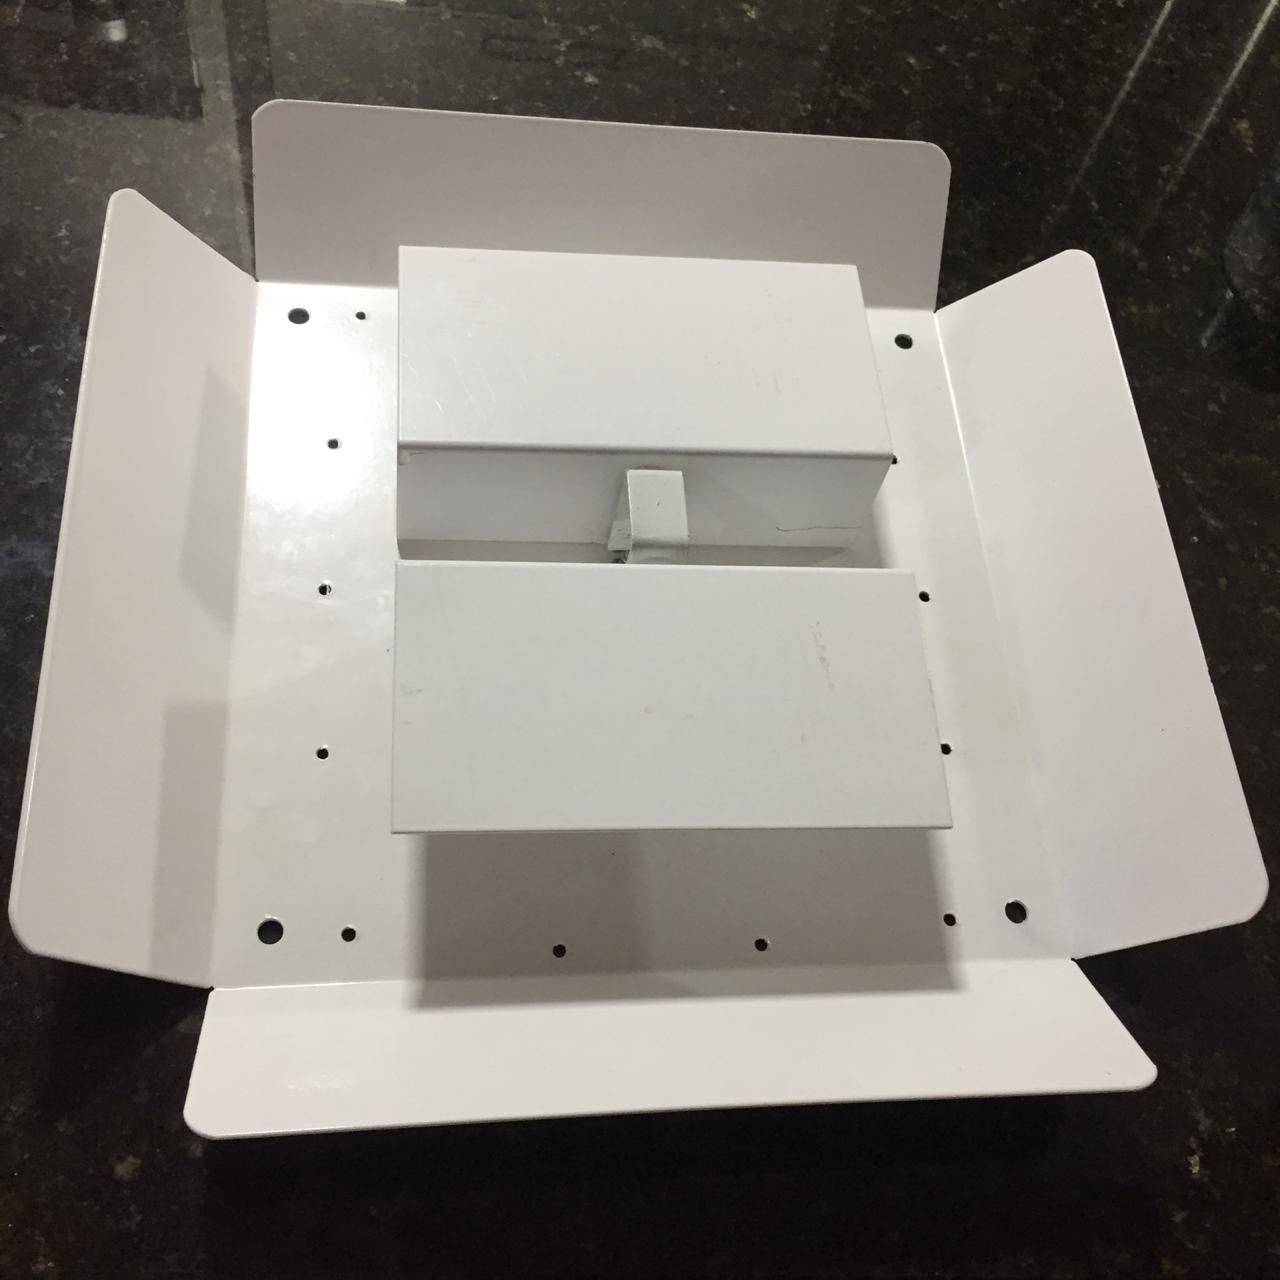
\includegraphics[scale = 0.15]{antena.jpeg}
   \caption{Antena dipolo com frequência central de 915MHz que será utilizada para a transmissão e recepção de dados no radar.}
   \label{antena}
    \end{figure}

Outros parâmetros importantes das antenas são sua diretividade, ou seja, a capacidade de focalizar energia em um ponto, e também o ganho da antena. Neste caso a antena possuiu um ganho e diretividade de 9dB, como mostrado na Figura \ref{ganho}.

\begin{figure}[H]
    \centering
   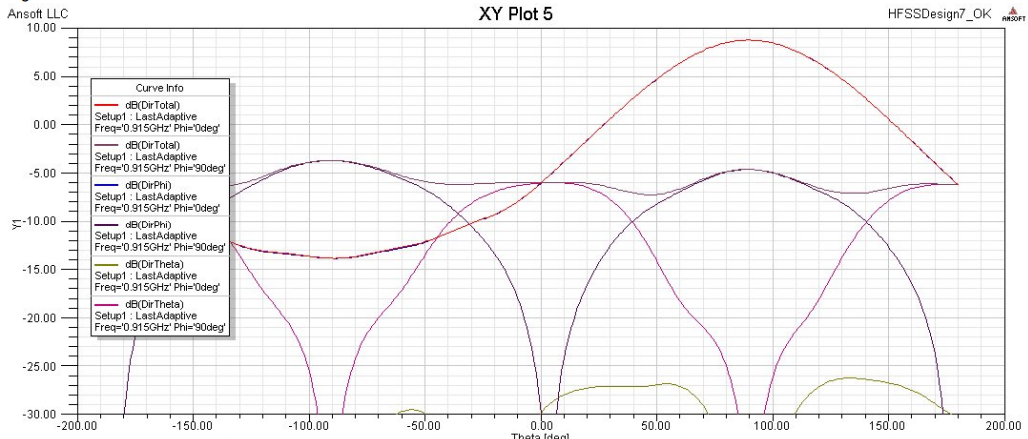
\includegraphics[scale = 0.45]{ganho.png}
   \caption{Diagrama de radiação com o ganho da antena.}
   \label{ganho}
    \end{figure}

Podemos verificar também a abertura 3 dB das antenas, onde está concentrado metade da energia transmitida ou recebida pela antena. Para calcular este ângulo é preciso pegar o maior valor no diagrama de radiação e deslocar 3 dB no eixo das ordenadas, sendo a abertura 3 dB a variação angular contida nessa região. Esse dado pode ser verificado tanto no diagrama disponibilizado pelo fabricante Figura \ref{ganho} onde se encontra na faixa dos 50$^{\circ}$ a 120$^{\circ}$ como no diagrama caracterizado em campo onde a mesma abertura se encontra na faixa de -35$^{\circ}$ a 35$^{\circ}$ de acordo com a Figura \ref{dr} confirmando que a antena utilizada possui uma abertura 3 dB de 70$^{\circ}$. 

\begin{figure}[H]
    \centering
   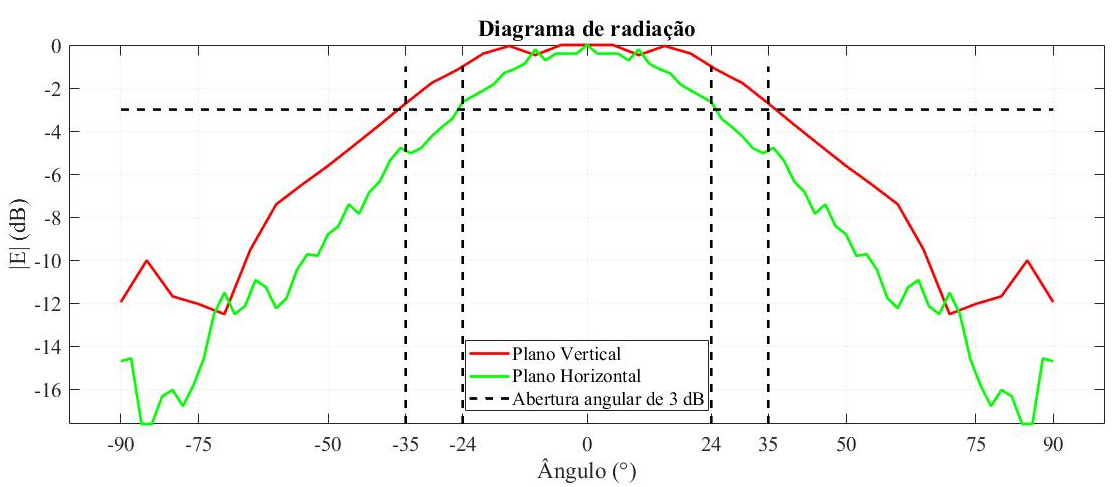
\includegraphics[scale = 0.3]{gir.png}
   \caption{Diagrama de radiação da antena e a
abertura 3 dB, caracterizada na faculdade.}
   \label{dr}
    \end{figure}


\subsection{Parâmetros do radar}


 Por se tratar de um radar que tem como objetivo mensurar a variação de frequência através do efeito \emph{Doppler}, um dos parâmetros necessários para se estabelecer o correto funcionamento do sistema é o cálculo da variação em frequência que se dá através da Eq. \ref{Doppler0} de efeito \emph{Doppler} \cite{young2009fisica}. 

\begin{equation}\label{Doppler0} 
  f_0 = f_f \Big(\frac{c \pm v_0}{c \mp v_f} \Big),
\end{equation} onde $f_0$ é a frequência observada pelo observador, $f_f$ é a frequência emitida pela fonte, \emph{c} é a velocidade da luz, $v_0$ é a velocidade do observador em relação ao meio, sendo esta positiva ao se aproximar da fonte e negativa ao se afastar, $v_f$ é a velocidade da fonte em relação ao meio, sendo positiva ao se afastar e negativa ao se aproximar do observador.
Como a velocidade do observador representa a velocidade do radar e o mesmo se encontra fixo na rodovia, então $v_0$ é considerado como sendo 0, resultando na Eq. \ref{Doppler0-1}.
%Nussenzveig, Moysés, H. Curso de Física Básica. [Minha Biblioteca]. Retirado de https://integrada.minhabiblioteca.com.br/#/books/9788521208044/
\begin{equation}\label{Doppler0-1} 
  f_0 = f_f \Big(1 + \frac{v_f}{c} \Big).
\end{equation}

A partir da relação $\Delta f = f_{f} - f_{0}$, podemos concluir que a variação de frequência é dada através da Eq. \ref{Doppler}.

\begin{equation}\label{Doppler} 
  \Delta f =  \frac{2v_f}{\lambda},
\end{equation} onde $\Delta f$ representa a variação de frequência do sinal, $v_f$ representa a velocidade relativa do alvo com relação ao radar e $\lambda$ é o comprimento de onda do sinal emitido pela antena. Como $\lambda$ depende exclusivamente da frequência do sinal emitido e o mesmo se encontra na faixa dos 915 MHz, utilizando a relação $f=c/\lambda$  podemos encontrar um valor para $\lambda$ de 0.328m. Substituindo na Eq. \ref{Doppler}, temos que $\Delta f = 6.1 Hz$.

De acordo com este resultado, uma variação de $1 m/s$ na velocidade da fonte para o radar é representada por um desvio de $6.1 Hz$. Utilizando uma variação em $km/h$ para representar a velocidade da fonte dividimos o resultado anterior por um fator de 3.6 de modo que uma variação de $1km/h$ pode ser visualizada através de um desvio de $1.7 Hz$.
Um outro fator importante para se estabelecer a variação em frequência é o ângulo entre a direção de transmissão/recepção do sinal e a trajetória do alvo, de modo que a equação \ref{Doppler} é alterada de acordo com o ângulo $\theta$ mensurado, mostrada na Eq. \ref{Doppler2} \cite{Radar}.
%http://www.radartutorial.eu/11.coherent/co06.en.html

 \begin{equation}\label{Doppler2} 
  \Delta f =  \frac{2v}{\lambda}cos \theta.
\end{equation}
Isso implica que a variação estabelecida na Eq \ref{Doppler} é dada como sendo a máxima para um alvo que se aproxima do radar. Quando o objeto se encontra muito distante do radar esse ângulo se torna muito pequeno e a varição causado por ele inexpressiva, porém de acordo com que o alvo se aproxima, pode ser um fator determinante no cálculo da velocidade do alvo.

Outro parâmetro é a distância máxima que o radar vai conseguir detectar um veículo, pois será necessário alertar ao motorista que vem em direção oposta a possibilidade de uma colisão frontal. Pois será necessário capturar a imagem do automóvel caso o mesmo ultrapasse a velocidade limite da via. De acordo com esses parâmetros foi definido uma distância de 100 m atendendo o tempo necessário para realizar os processos embarcados no totem, entre eles o cálculo da velocidade do veículo e o comando para captura da imagem. Uma vez estipulada a distância máxima para captura foi possível realizar o cálculo dos demais parâmetros.

%%%%%%%%%parametrôs de potencia e ruido%%%%%%%%%%%%%%
A Eq. \ref{potencia_recebida} define a potência a ser recebida em função do ganho da antena, distância do alvo, da potência transmitida, do comprimento da onda transmitida e da área de seção transversal do alvo. \textcolor{red}{4}\cite{Richards}:
\begin{equation}\label{potencia_recebida}
    P_t\, =\,   P_r \frac{(4\pi)^{3}\,  R^{4}}{G^{2}\,   \lambda^{2}\, \sigma }.
\end{equation}%

Onde $P_t$ é a potência transmitida, $P_r$ a potência recebida, $G$ o ganho da antena, $\lambda$ o comprimento de onda do sinal a ser enviado, $\sigma$ a área de seção transversal média do alvo e $R$ a distância do alvo até a antena.

Através das informações acerca da USRP-NI2901 \cite{RDS}  a potência miníma no canal de recepção RX é de -85 dBm, porém para realização dos cálculos foi estipulado uma sinal na recepção com potencia de -50 dBm utilizando os dados onde: $R=100 \, m$, $G=9 \, dB$ Fig.\ref{antena}, $\lambda=0.328 \, m$ Eq\ref{Doppler} e $\sigma=1 \, m^{2}$ \cite{Richards}. A partir desses dados e da Eq. \ref{potencia_recebida} podemos chegar a um resultado de $P_t=14.66 \, dBm$ de potência serão necessário para enviar o sinal a um alvo localizado a 100m.

A potência de ruído térmico, predominante no projeto é definida na Eq. \ref{potencia_ruido}, onde $P_n$ é a potência de ruído, definida no receptor, $k$ a constante de Boltzman = $1.38 \times 10^{-23} \, J/K$ , $T_e$ a temperatura equivalente de ruído e $B$ a largura de banda. \textcolor{red}{4}

\begin{equation}\label{potencia_ruido}
    P_n = k\, T_e\,B.
\end{equation}

A temperatura equivalente de ruído, $T_e$, corresponde a soma da temperatura equivalente de ruído da antena, aqui estimada como temperatura ambiente, 290 K, com a temperatura equivalente de ruído do sistema eletrônico, aqui considerados a relação entre figura de ruído e temperatura equivalente de ruído para obter, no final, uma temperatura equivalente de ruído do sistema de 1453 K. De acordo com esses dados encontrou-se uma potência de ruído para o sistema de -121 dB.
\subsection{Processamento de sinais}

A Figura \ref{processos_geral_radar} mostra o funcionamento geral de um sistema de radar utilizando uma \emph{Raspberry Pi 3} e um Rádio Definido por Software (RDS) que é um sistema com componentes físicos em  \emph{Hardware}, que porém utiliza da flexibilidade de softwares para a implementação  de seus componentes, com isso possibilitando uma gama muito maior de aplicações. Será utilizado o  modelo \emph{Universal Software Radio Peripheral} - USRP vista na Figura \ref{processos_geral_radar}.



\begin{figure}[H]
    \centering
    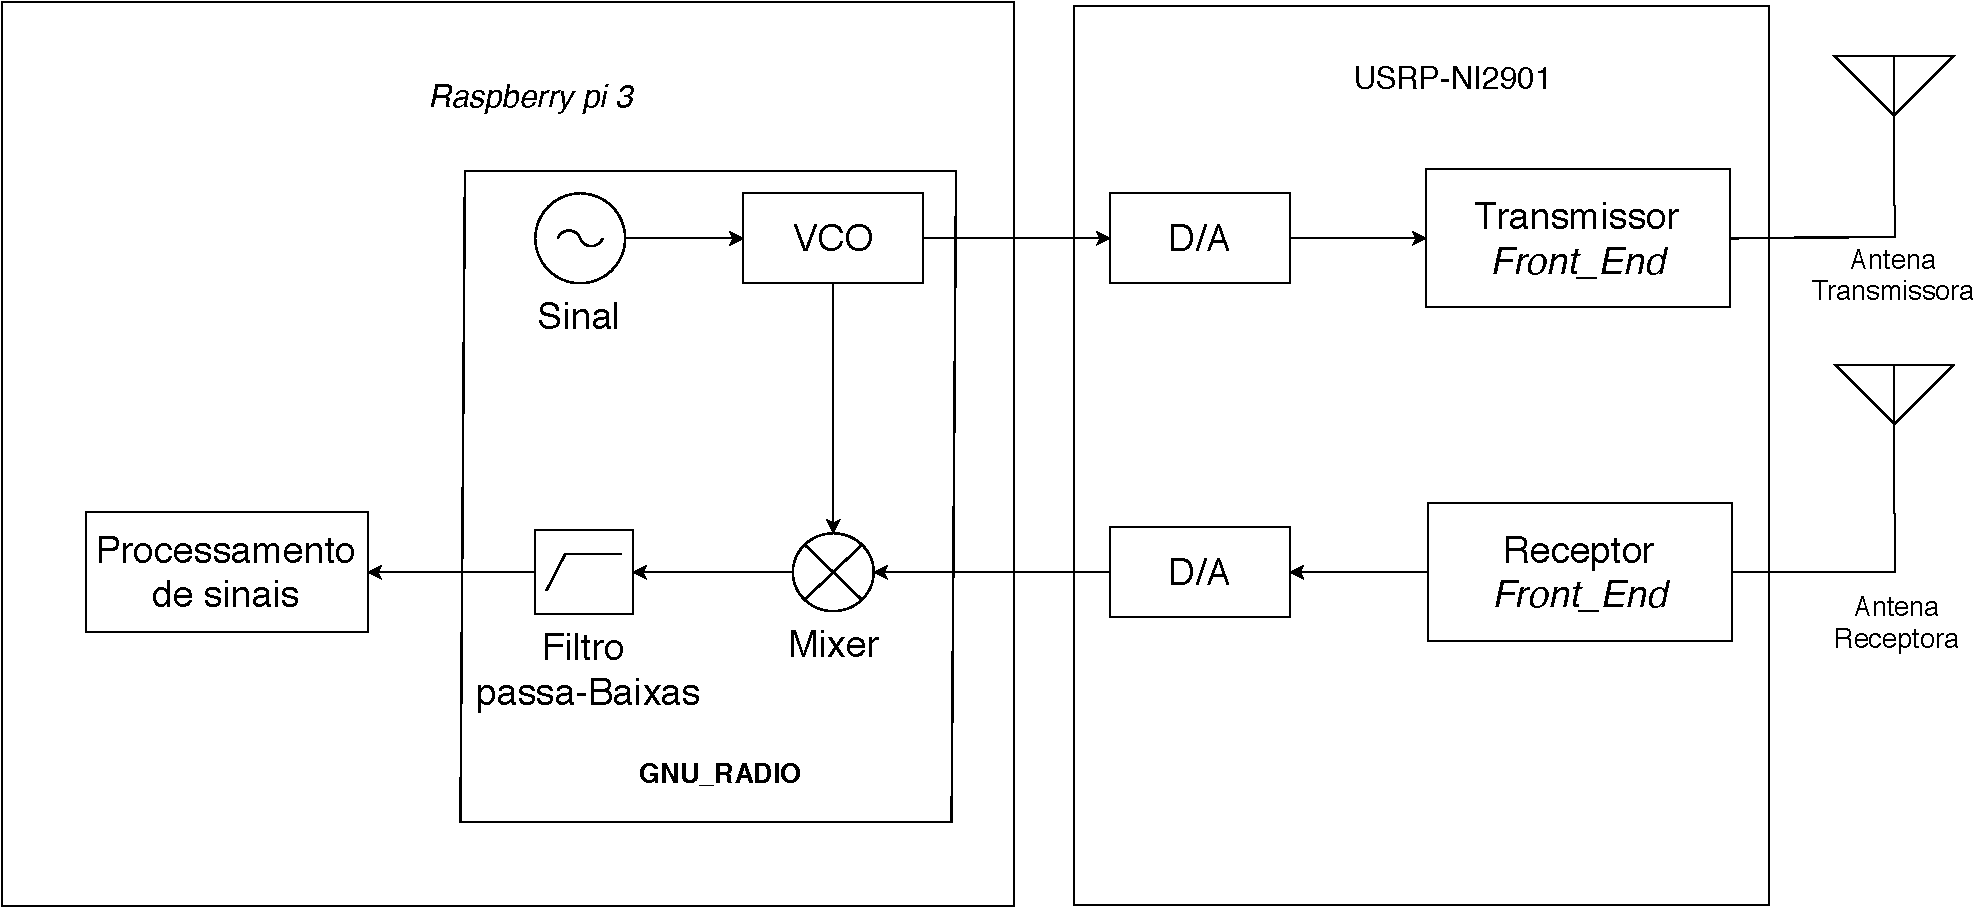
\includegraphics[scale=0.35]{diagrama_radar2.pdf}
    \caption{Diagrama do radar utilizado na implementação através do software GNU Rádio.}
    \label{processos_geral_radar}
\end{figure}

Será utilizado o GNU-RADIO um software de código aberto que fornece blocos de processamento de sinais para implementação em RDS. O software será embarcado em um microcontrolador \emph{Raspberry Pi 3} que através do GNU-RADIO enviará e receberá os sinais, após a recepção o sinal será processado no microcontrolador e calculado o desvio de frequência para então ter a velocidade do veículo. 


O sinal da portadora escolhido de acordo com a Figura \ref{processos_geral_radar} é modulado no bloco \emph{VCO - Voltage-Controlled Oscillator}, no qual o sinal oscila através de uma frequência central e de acordo com a sensibilidade do VCO e a amplitude da portadora variam com o tempo fazendo com que a frequência central seja deslocada. Esses dados são enviados da \emph{Raspberry Pi 3} para o USRP através do protocolo de comunicação UART, onde os dados são convertidos de digital para analógico e executados pelo USRP, que através do bloco \emph{front-end} transmissor envia o sinal para antena. Após o sinal se propagar em espaço livre, ser refletido por um objeto e captado pela antena receptora,  é enviado para o bloco \emph{front-end} receptor e depois convertem os dados de analógico para digital, mandando de volta a \emph{Raspberry Pi 3} para o GNU-RADIO passando por um \emph{mixer} e após uma filtro passa-baixas para pegar o desvio de frequência, por fim, o sinal é tratado para obter o cálculo da velocidade.



A resolução de velocidade depende diretamente da resolução em frequência do sinal após a \emph{Fast Fourier Transform} (FFT), que depende da quantidade de amostras adquiridas e da frequência de amostragem, como demosntrado pela Eq.:
\begin{equation}\label{resolucao_freq}
    \Delta f = \frac{f_{s}}{2\,N}.
\end{equation}
Onde N é a quantidade de amostras adquiridas, $f_{s}$ a frequência de amostragem e $\Delta f$ a resolução em frequência. A partir da Eq. \ref{resolucao_freq} definiu-se o parâmetro da frequência de amostragem necessária para garantir 
uma resolução de 1,7 Hz para uma determinada quantidade de amostras, neste projeto 1024 amostras, resultando em 870 Hz para o sinal a ser enviado.

\subsection{GNU-RADIO}

    Como mencionado, para implementação do sistema de radar FMCW foi utilizado o GNU-RADIO de acordo com a Figura \ref{processos_geral_radar}, de modo que o digrama obtido pelo software está descrito de acordo com a Figura \ref{GNU}

\begin{figure}[H]
    \centering
    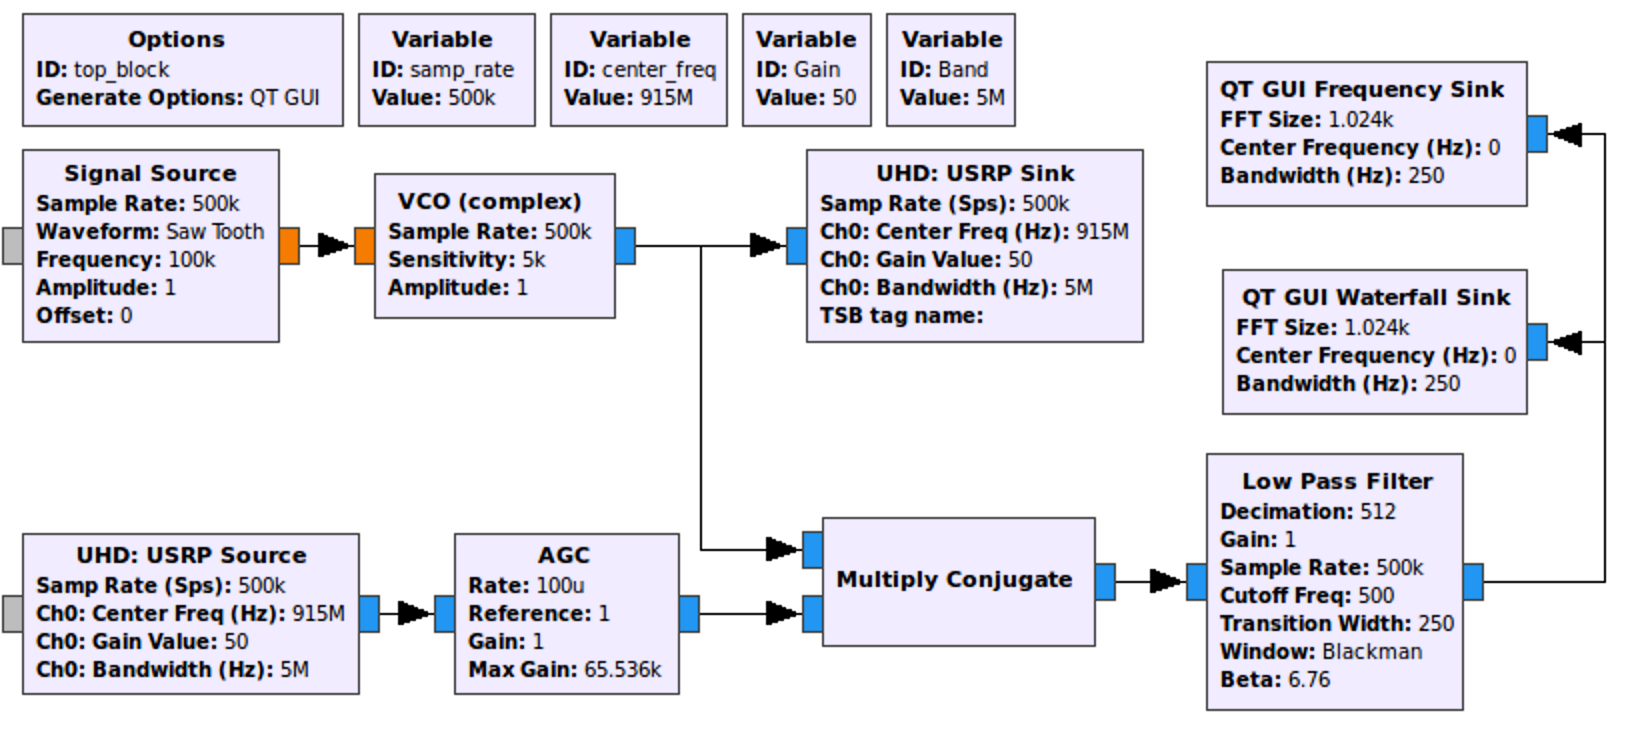
\includegraphics[scale=0.4]{GNU.png}
    \caption{Diagrama do radar utilizado na implementação através do software GNU Rádio.}
    \label{GNU}
\end{figure}


\begin{itemize}
    \item \emph{Signal Source}: Bloco que representa o sinal a ser modulado, utilizando um sinal do tipo dente de serra com uma frequência de 100 KHz e amplitude de 1V.
    \item \emph{VCO (complex):} Bloco que realiza a modulação da portadora na frequência central de 500 KHz e possui uma sensibilidade de 5 KHz, fazendo com que a frequência do sinal varie de 495 KHz a 505 KHz.
    \item \emph{UHD USRP Sink:}  Responsável por realizar o \emph{upconverter} do sinal de entrada para frequência central da antena que foi definido como 915 MHz com uma largura de banda de 5 MHz.
    \item \emph{UHD USRP Source:} Responsável por realizar o \emph{downconverter} do sinal que é captado pela antena, possibilitando com que o mesmo seja processado pelo software.
    \item \emph{AGC:} Ganho controlado para manter o sinal de saída da antena receptorana mesma margem de tensão do sinal de entrada.
    \item \emph{Multiply Conjugate:} Realiza a convolução do sinal modulado pelo VCO com o sinal recebido pela antena, fazendo com que a frequência central seja deslocada para mais ou menos em relação a frequência da portadora movendo-a para zero e também para duas vezes a frequência da portadora.
    \item\emph{Low Pass Filter:} Faz com que somente a informação presente em torno da frequência zero seja preservada, fazendo com que seja mais visível a variação de frequência uma vez que a banda utilizada foi de 500 Hz com uma janela do tipo \emph{Blackman}.
    \item \emph{Waterfall Sink:}Modo de visualização no qual o desvio de frequência pode ser visualizado mais facilmente.
    \item \emph{Frequency Sink:}Modo de visualização onde os índices de frequências podem ser visualizados.
\end{itemize} 

\subsection{Testes e resultados}

    Foram realizados dois testes para validação do sistema do radar. O primeiro teste consistiu em realizar um experimento em campo para captação do movimento de um automóvel através do desvio de frequência da recepção em relação à frequência transmitida, sendo esta última deslocada para zero com o intuito de se visualizar somente sua variação no momento em que o veículo se aproxima a uma distância de 20 metros. O resultado do teste é mostrado na Figura \ref{TVeiculo}

\begin{figure}[H]
    \centering
    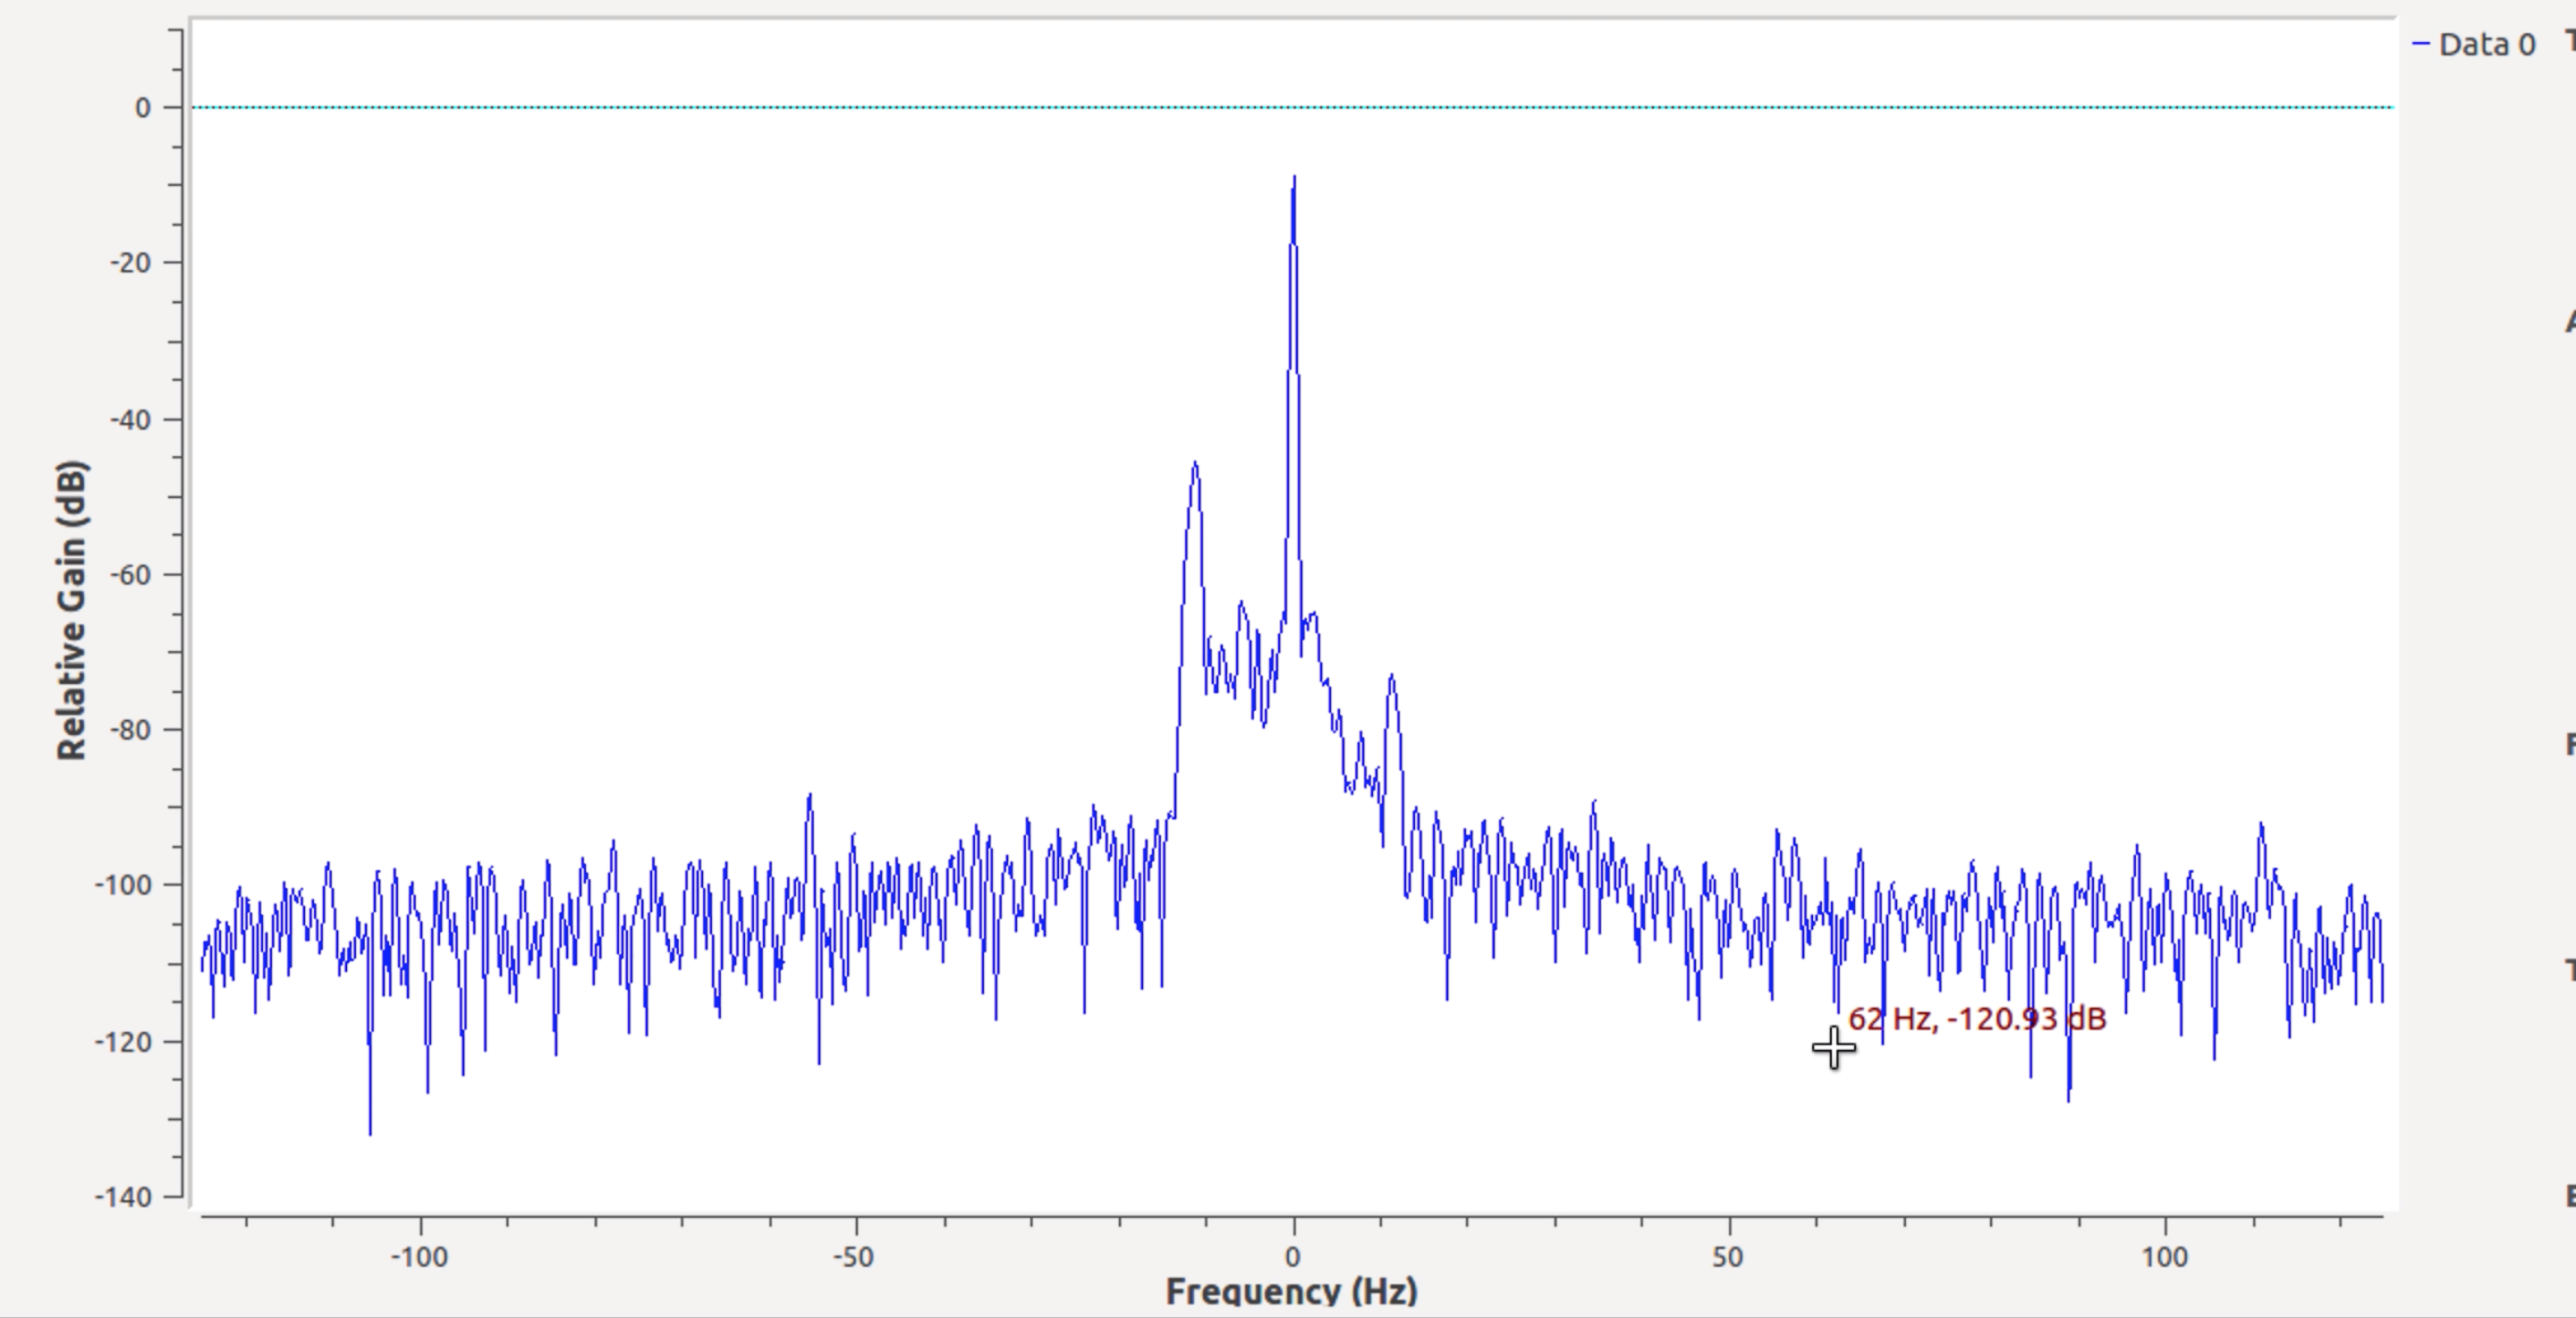
\includegraphics[scale=0.23]{Carro.png}
    \caption{Gráfico ilustrando o desvio de frequência causado pela captura de um veículo em movimento.}
    \label{TVeiculo}
\end{figure}

A Figura \ref{TVeiculo} mostra a FFT da recepção do sinal no momento o qual o carro se aproxima do radar,
onde no centro temos o pico de maior ganho que representa frequência de transmissão de 915MHz na qual a antena está transmitindo, e o pico secundário dentro da FFT representa a o deslocamento em frequência causado pelo movimento do carro, e de acordo com essa variação e utilizando a equação \ref{Doppler} é possível estabelecer a velocidade do mesmo pelo radar.
Com isso foi possível validar a transmissão e recepção do sinal à distância estipulada na seção de cálculos do radar. 

O segundo teste realizado com o radar consistiu em
medir a variação de velocidade radial na qual um sinal refletido por um ventilador é captado pela antena, por se tratar de uma velocidade angular irá aparecer no espectro do sinal várias frequências que estão relacionadas com a velocidade linear do ventilador ao longo da pá do mesmo, como mostrado nas Figuras \ref{Vel0} a \ref{Vel3}.


\begin{figure}[H]
    \centering
    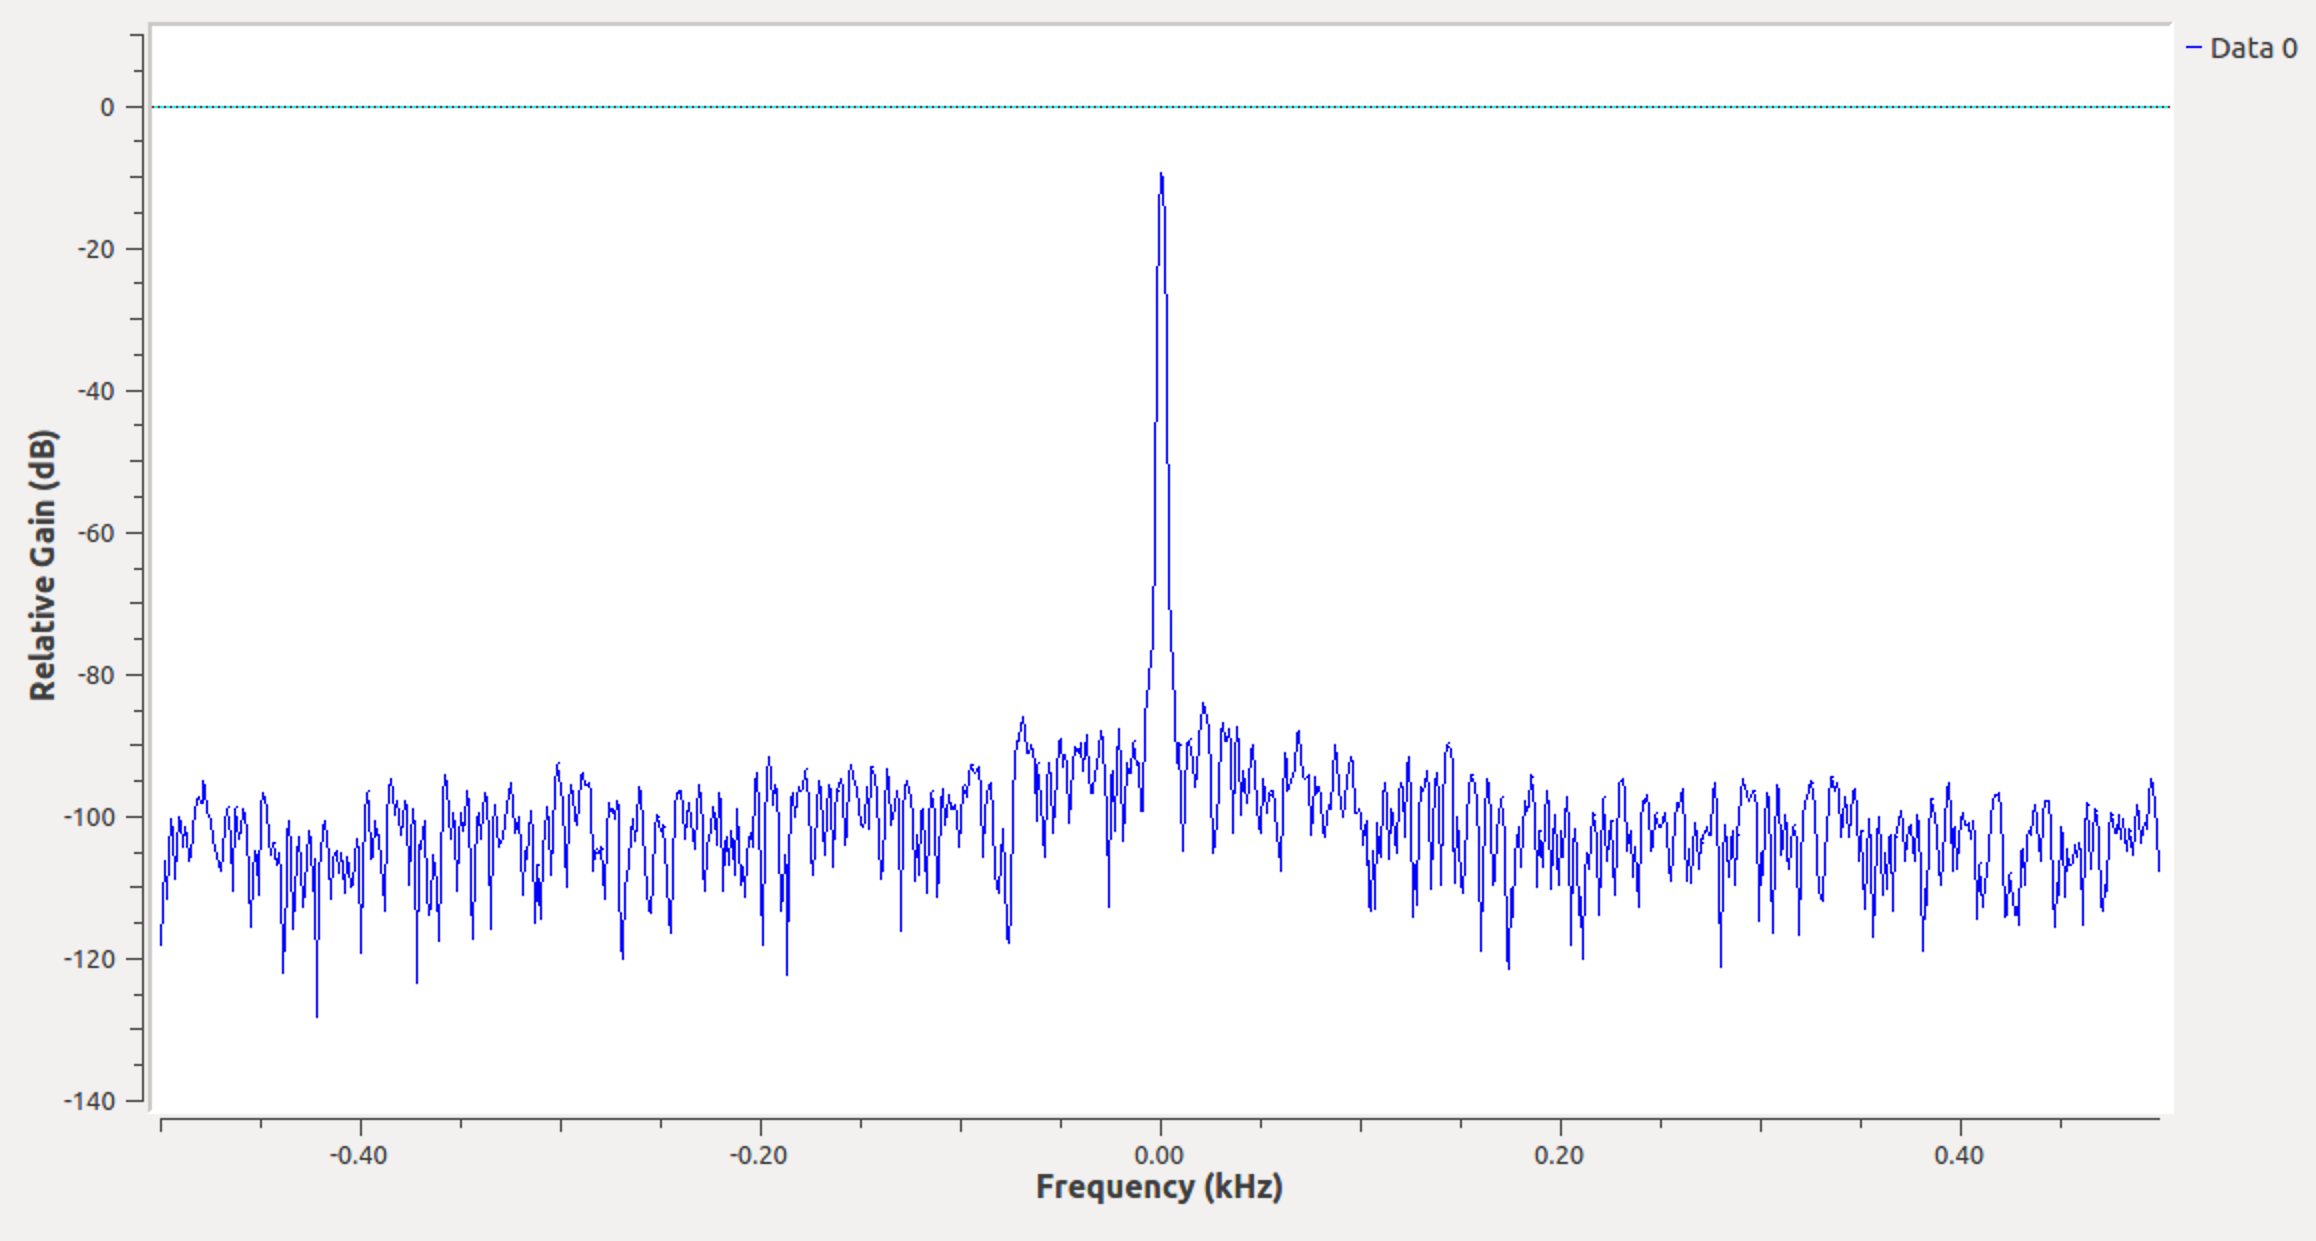
\includegraphics[scale=0.3]{Ventilador_desligado.png}
    \caption{Imagem da captação do radar com o ventilador desligado.}
    \label{Vel0}
\end{figure}

\begin{figure}[H]
    \centering
    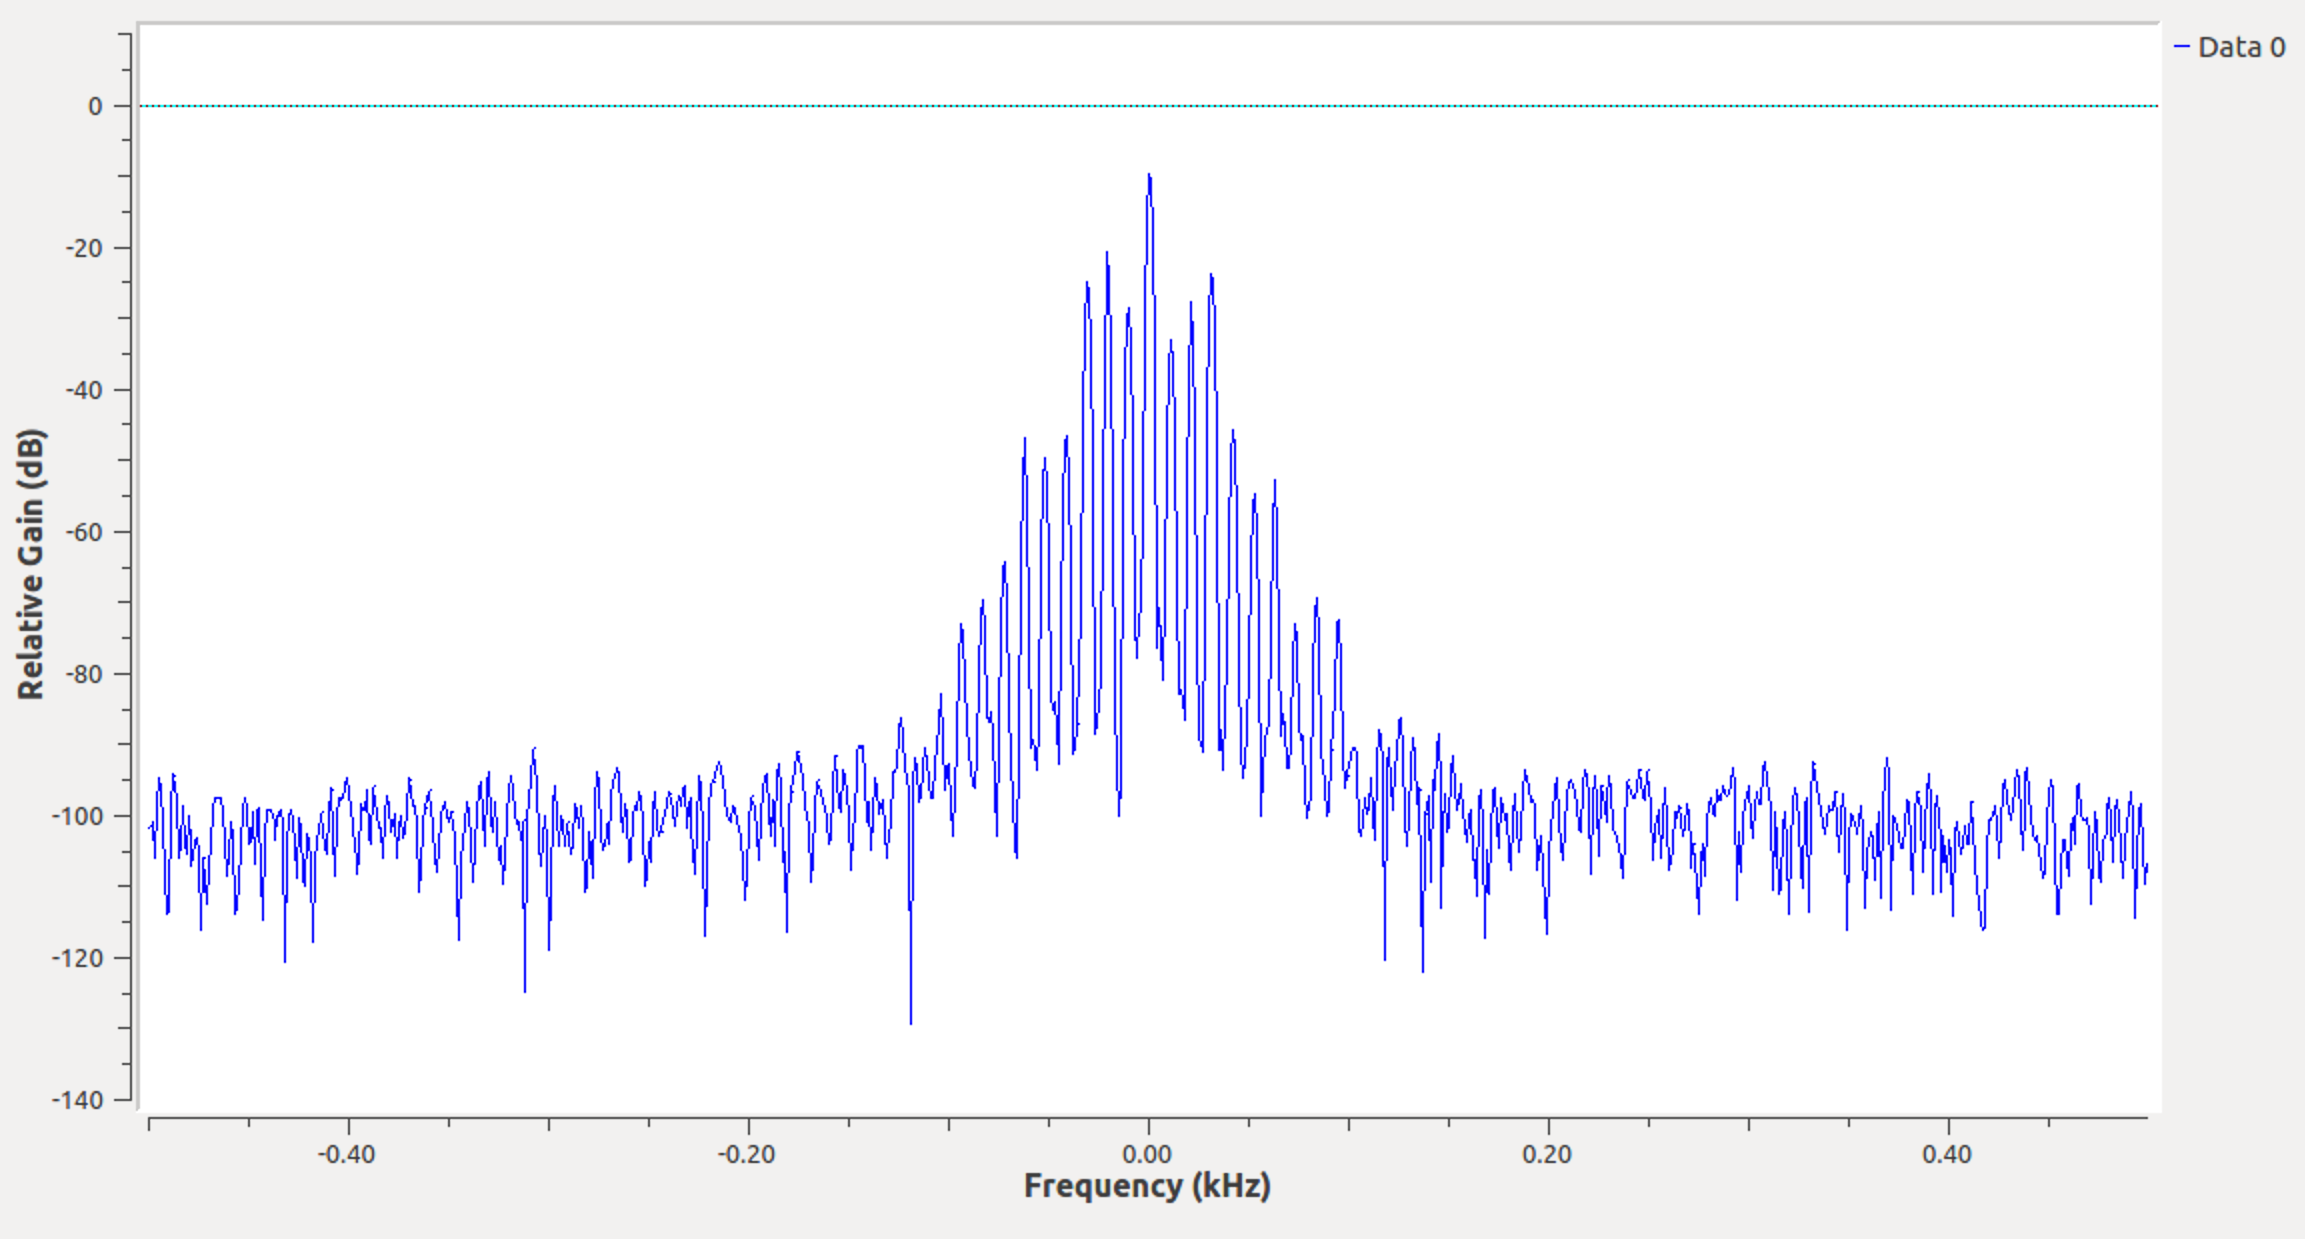
\includegraphics[scale=0.3]{Ventilador_vel1.png}
    \caption{Imagem da captação do radar em velocidade 1.}
    \label{Vel1}
\end{figure}
      
\begin{figure}[H]
    \centering
    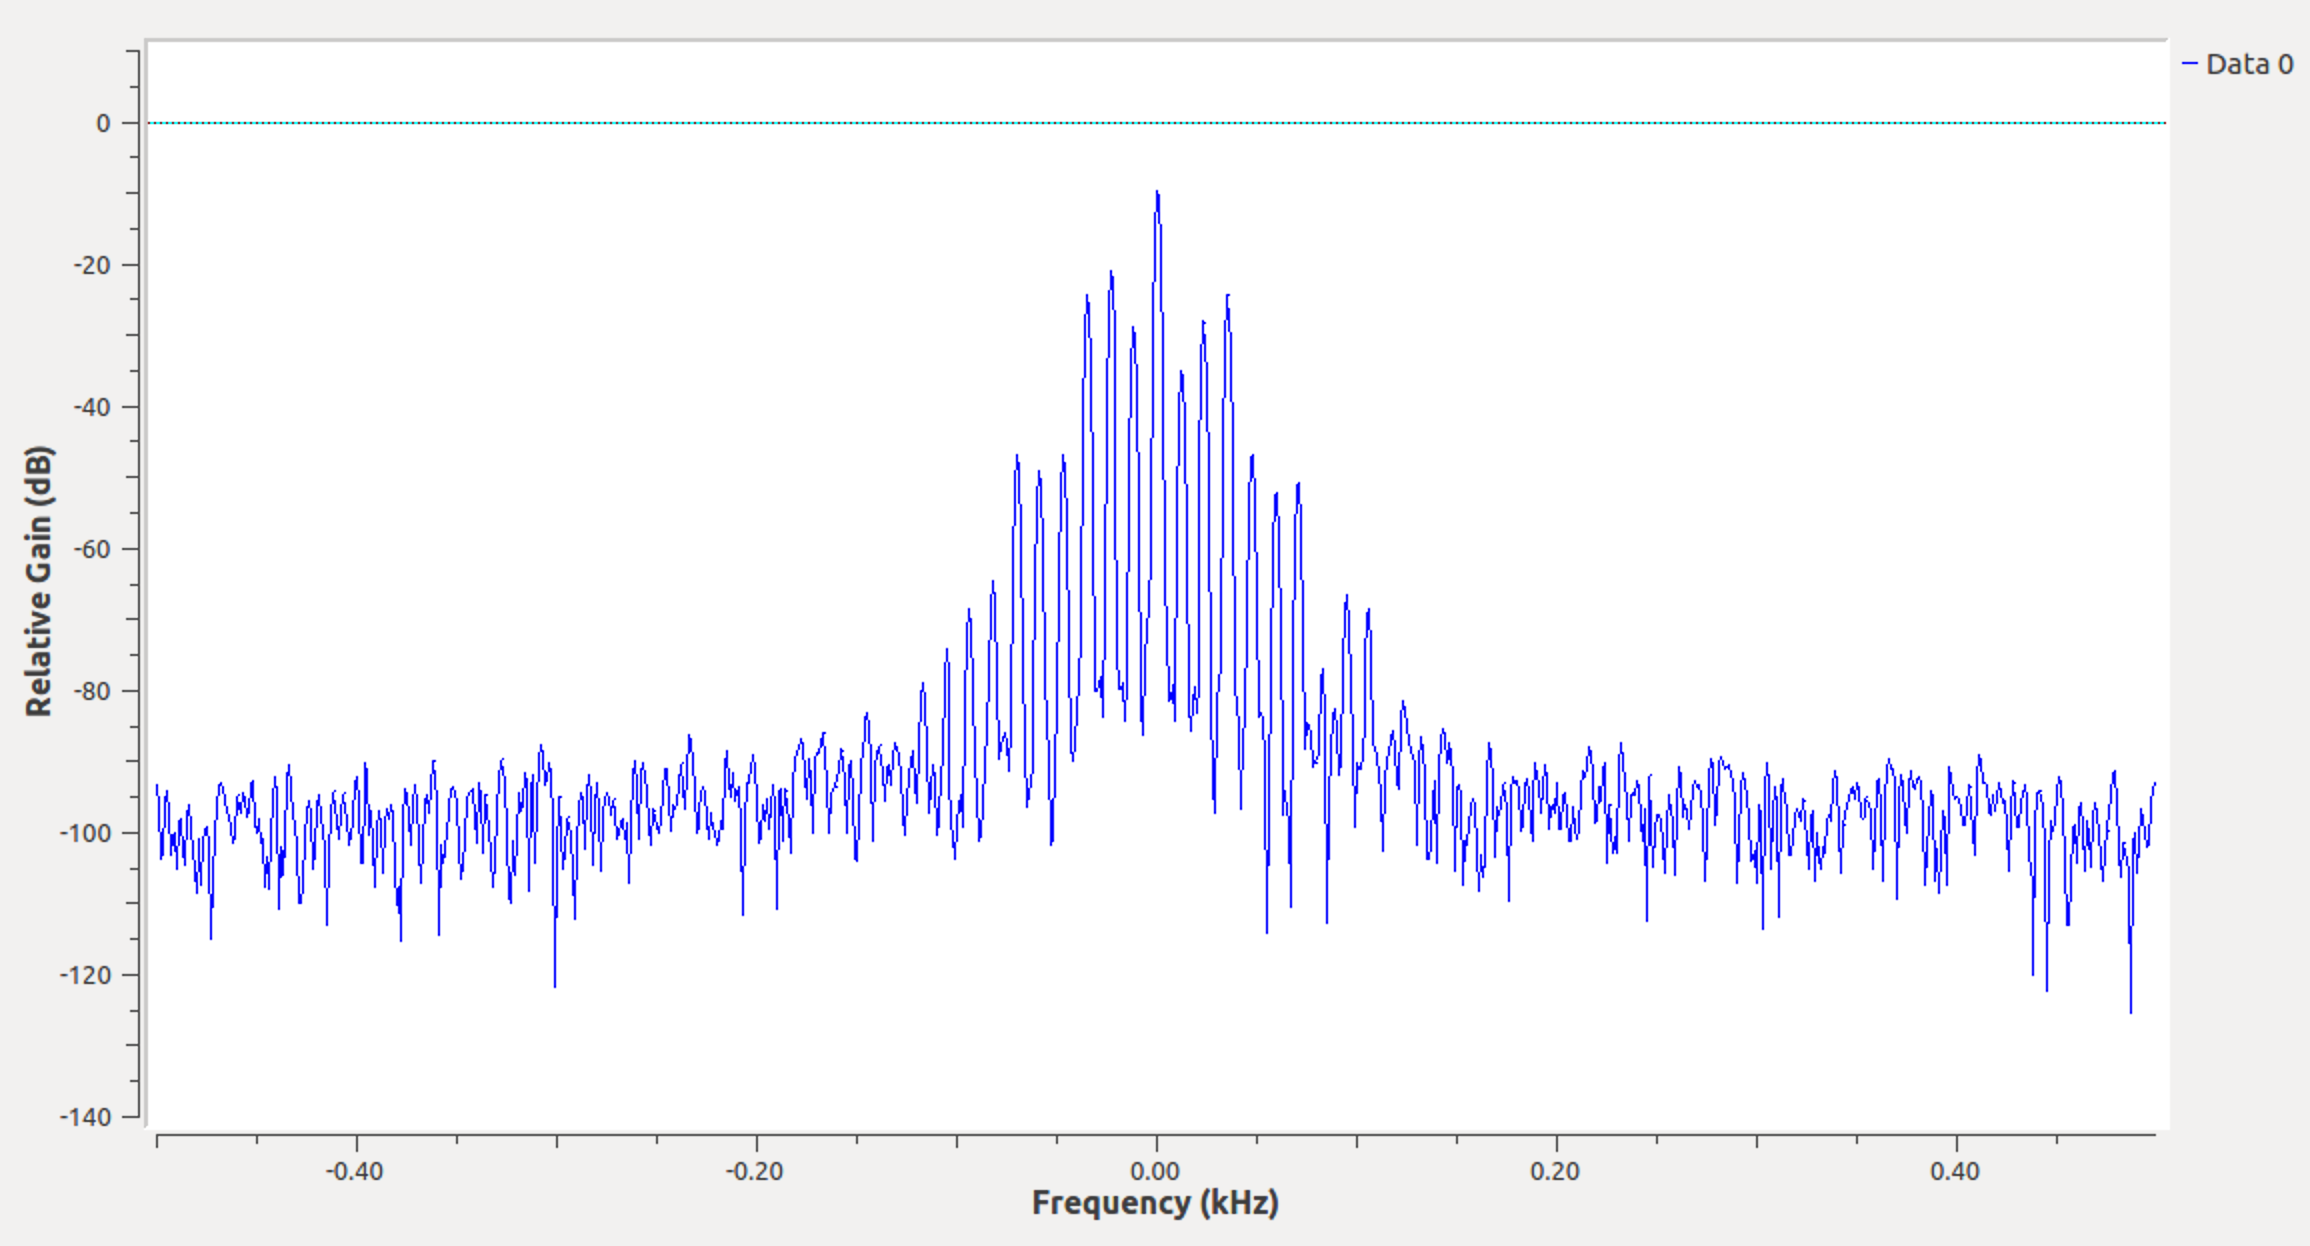
\includegraphics[scale=0.3]{Ventilador_vel2.png}
    \caption{Imagem da captação do radar em velocidade 2.}
    \label{Vel2}
\end{figure}

\begin{figure}[H]
    \centering
    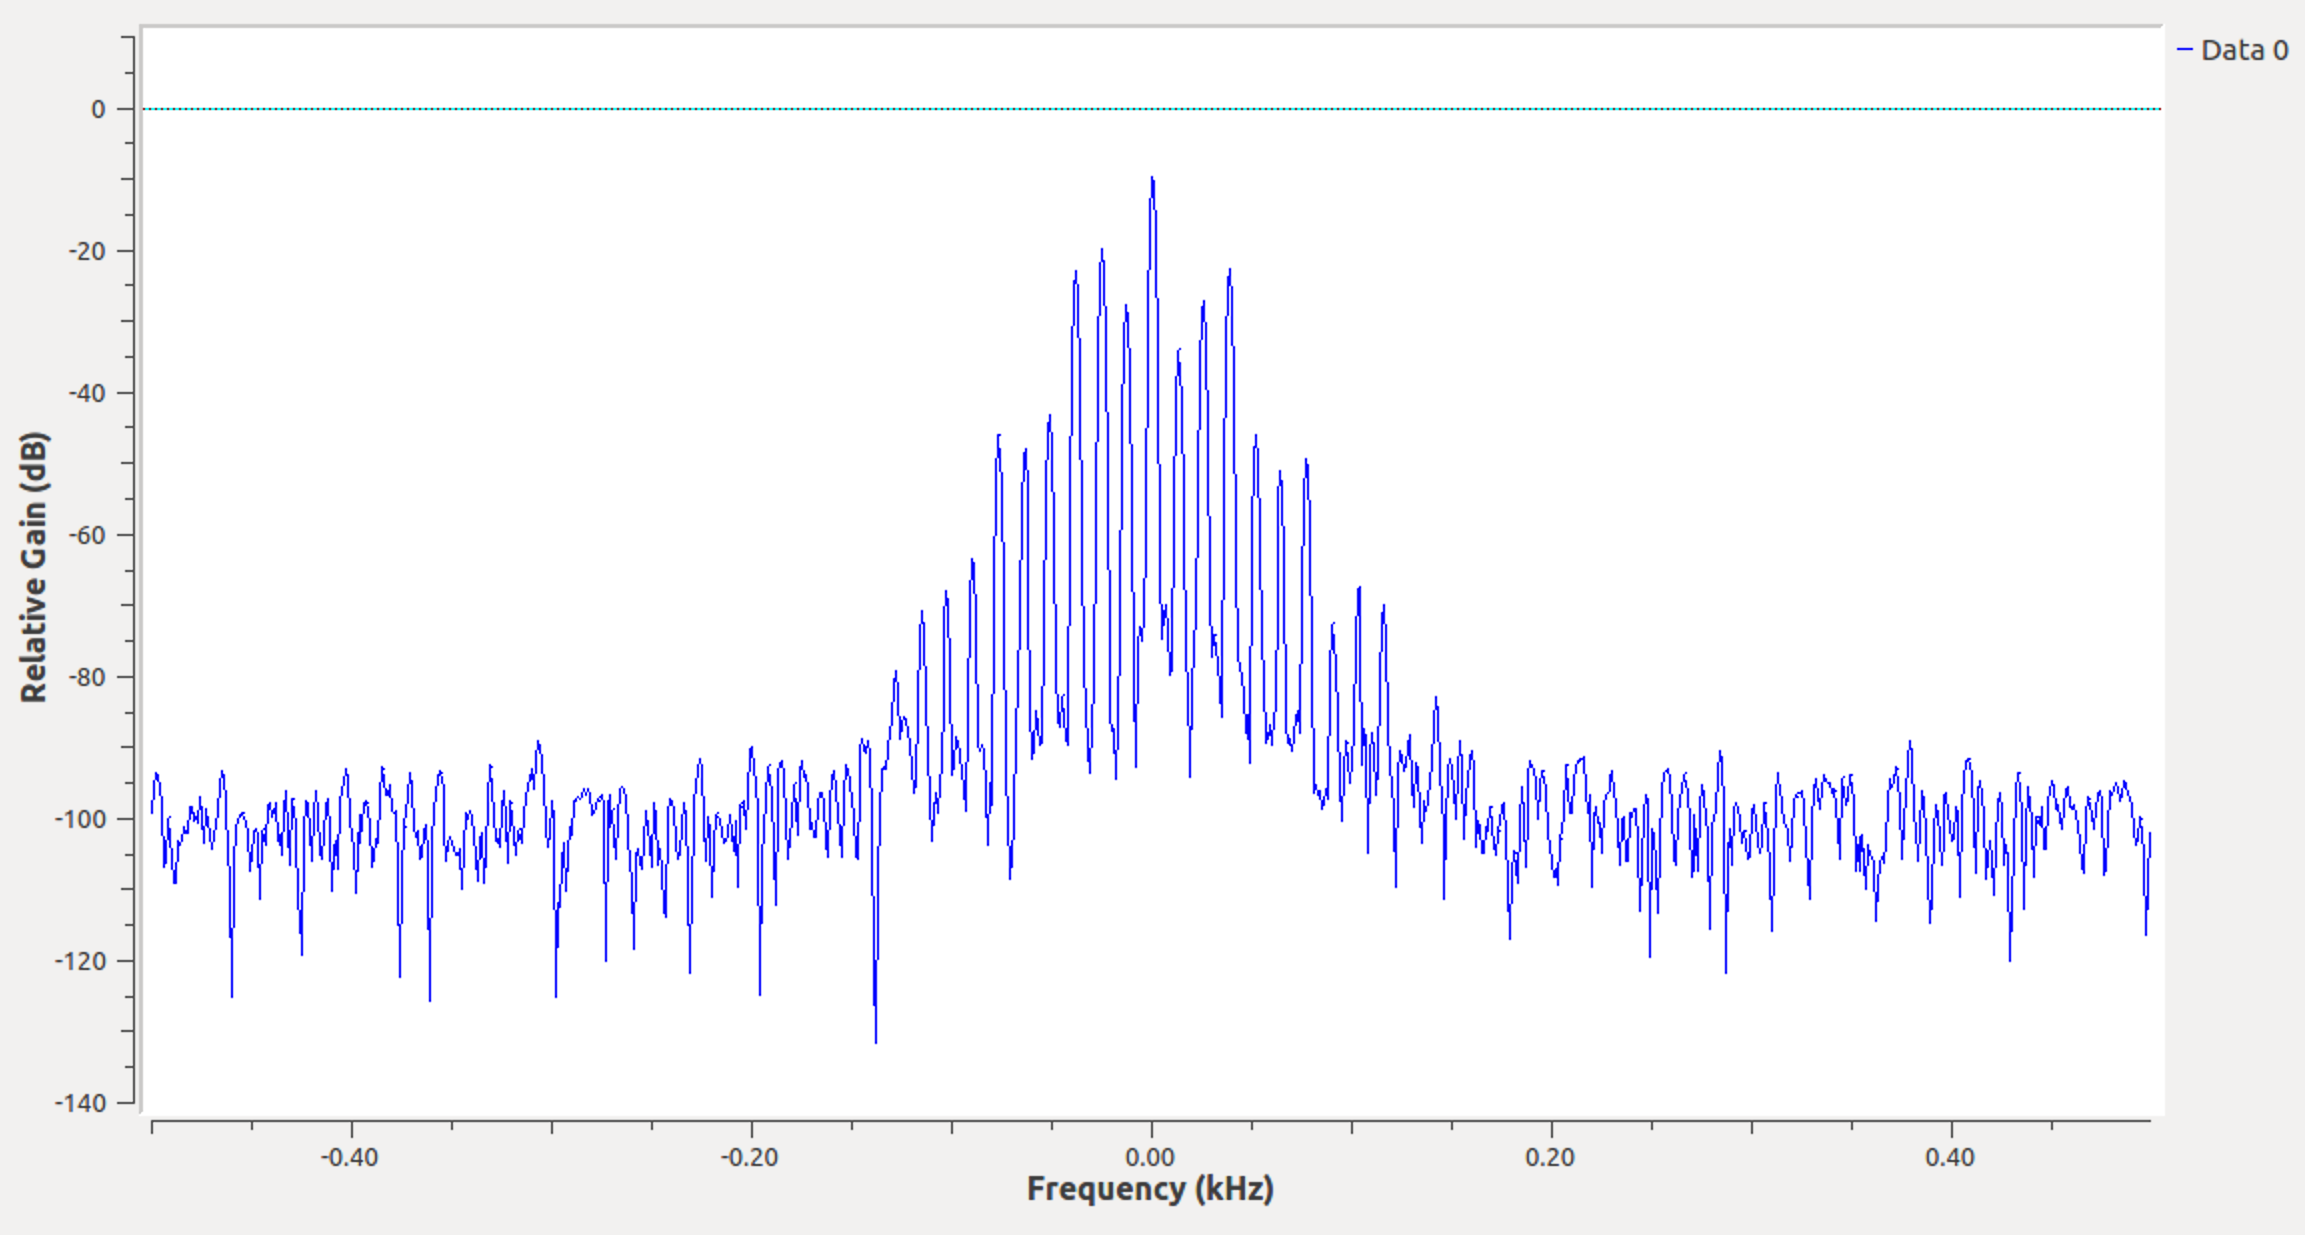
\includegraphics[scale=0.3]{Ventilador_vel3.png}
    \caption{Imagem da captação do radar em velocidade 3.}
    \label{Vel3}
\end{figure}

De acordo com o a Figura \ref{Vel0} onde pode ser verificado somente um pico na frequência de transmissão da antena, concluindo que não ha nenhum objeto com velocidade radial próximo do radar. Já na Figura \ref{Vel1} pode verificar um espalhamento espectral do sinal na recepção, pelo fato de que quando o sinal refletir sobre o ventilador a antena irá captar um grande número de velocidades devido ao aumento gradual da velocidade linear de acordo com que o sinal refletido está mais afastado do centro do ventilador fazendo com que isso seja enxergado como um espalhamento na FFT do sinal na recepção. De acordo como são analisadas as Figuras \ref{Vel2} e \ref{Vel3}, pode-se notar a expansão do espalhamento espectral devido ao aumento da velocidade angular do ventilador.


%%%%%%%%%%%%%%%%%%%%%%%%%%%%%%%%%%%%%%%%%%%%%%%%%%%%%%%%%%%%%%%%%%%%%%%%%%%%%%%%%%%%%%%%%%%%%%%%%%%%%%%%%%%%%%%%%%%%%%%%%%%%%%%%%%%%%%%%%%%%%%%%%%%%%
        
\section{Sistema de controle}

O sistema de controle tem como função principal realizar o processamento de imagens, monitoramento e comunicação dos vários módulos presentes no projeto. Os sistemas foram embarcados em um microprocessador \emph{Raspberry Pi 3}, onde a Figura \ref{redepetri} mostra o diagrama de estados do sistema em rede Petri no software PIPE. A \emph{Raspberry pi 3} foi escolhida pelo seu alto desempenho com relação ao tempo de processamento dos sinais que serão enviados, por atender a todos os protocolos de comunicação a serem feitos com os módulos escolhidos e também por apresentar um bom custo-beneficio.

\begin{figure}[H]
    \centering
    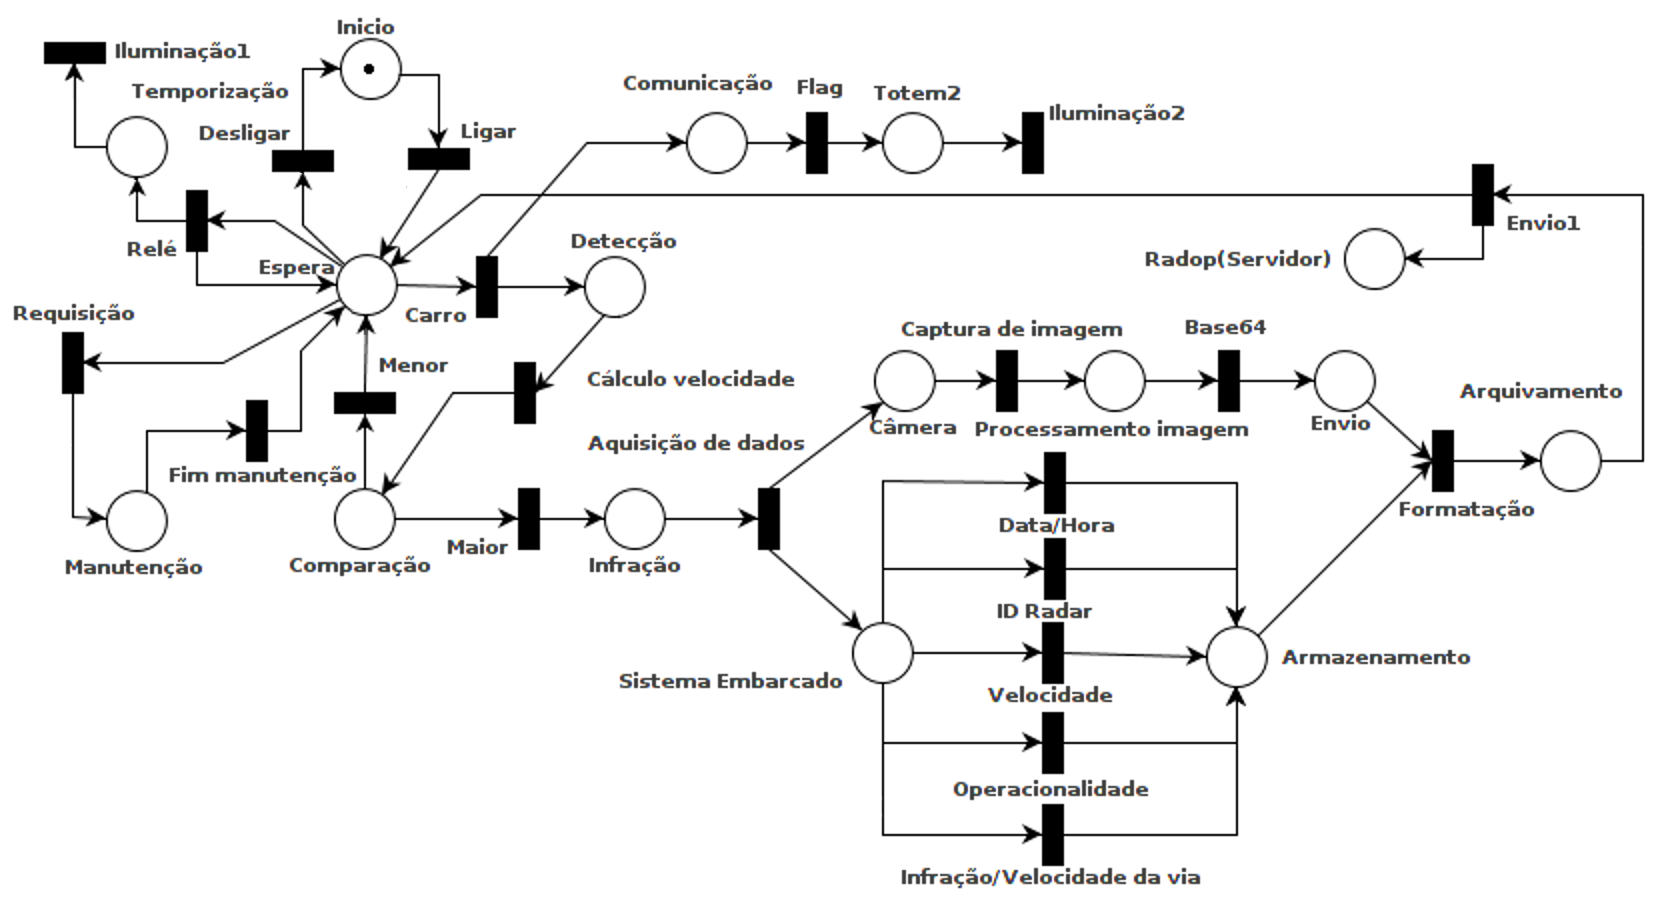
\includegraphics[scale=0.5]{Petri.png}
    \caption{Rede de petri para a solução proposta para o sistema eletrônico, feito no software PIPE.}
    \label{redepetri}
\end{figure}

A Figura \ref{comunicacao} mostra o diagrama de conexão dos diferentes módulos do projeto ligados ao microcontrolador \emph{Raspberry pi 3}, além disso mostra as alimentações e os protocolos de comunicação utilizados por cada um dos componentes.

     \begin{figure}[H]
    \centering
   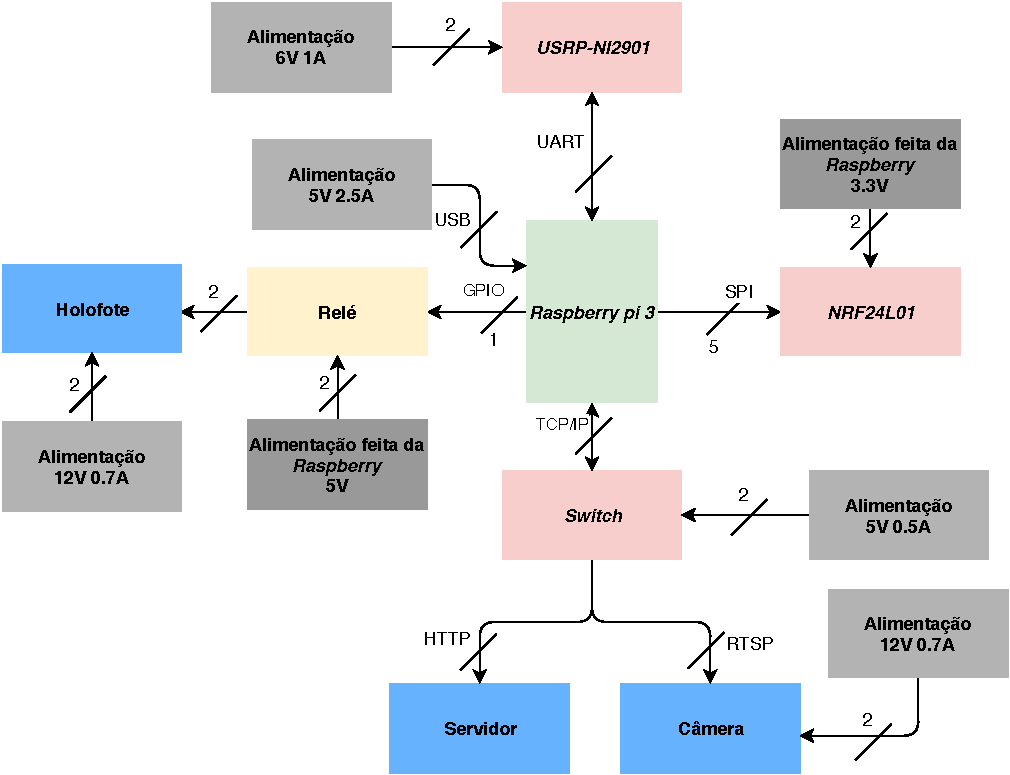
\includegraphics[scale = 0.75]{sistema_controle.pdf}
   \caption{Diagrama lógico do sistema de controle do projeto, onde o microprocessador \emph{Raspberry Pi 3} controla os demais sistemas e faz a comunicação. Dentre as comunicações estão o servidor, o sistema de sinalização e o sistema de comunicação entre os totem, além do controle de captura de imagem com a câmera e o pré-processamento da imagem.}
   \label{comunicacao}
    \end{figure}
    
\subsection{Tempo de latência}\label{tempo_latencia}

Dentre os principais requisitos solicitados pelo microprocessador é que deve possuir uma latência máxima de operação para se comunicar entre os módulos de aproximadamente 1.36 segundos, sendo este dado obtido através do tempo em que um veículo com velocidade máxima de 150 km/h usaria para percorrer a distância do ponto de captura de sua velocidade, no máximo a 50 metros antes do radar, até o ponto onde ocorre a captura da imagem, a 7 metros após o radar, caso ocorra uma infração. 
      
\subsection{Sinalização}
    
Quando o veículo se aproximar do radar, será enviado uma informação para o outro totem avisando ao condutor que um automóvel está se aproximando em direção oposta. O totem no qual recebeu a informação acionará um aviso luminoso, para que o condutor tenha uma atenção redobrada na curva. Após a detecção, a \emph{Raspberry Pi 3} através do módulo \emph{Wi-fi} NRF24L01 transmitirá uma \emph{flag} para o outro totem que faz a recepção da informação. Ao receber essa informação, o sistema de controle envia um sinal para um relé que fará o chaveamento para ligar o aviso luminoso por 10 segundos, sendo que o mesmo será atualizado se for detectado outro carro durante o intervalo, alertando o condutor sobre um veículo se aproximando na direção contrária. Esse tempo de 10 s de iluminação é necessário pelo fato do tempo em que o veículo leva para ser detectado até passar pela curva, usando o pior caso do veículo a 150 km/h em uma curva de 200 m.
A Figura \ref{esquematico} mostra o esquemático do sistema de sinalização, onde são feitas as conexões entre o módulo \emph{NRF24L01}, a \emph{Raspberry Pi 3} e o relé que ligará o holofote.

\begin{figure}[H]
    \centering
    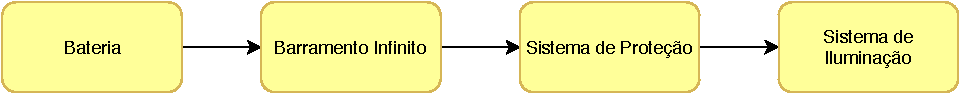
\includegraphics[scale = 0.8]{esquematico.pdf}
    \caption{Esquemático do sistema de sinalização do radar, que é composto pelo o módulo \emph{NRF24L01} a \emph{Raspberry Pi} e o relé, onde o módulo recebe e transmite o sinal com o outro totem e o microprocessador que aciona através do relé o holofote para fazer a sinalização. Foi utilizado a ferramenta fritzing.}
    \label{esquematico}
\end{figure}
   
O protocolo que fará a comunicação entre a \emph{Raspberry Pi} e o módulo NRF24L01 é o \emph{Serial Peripheral Interface} (SPI). Este módulo foi escolhido por ter um baixo consumo de energia, um alcance de sinal de 1 km de distância com outro totem e por sua taxa máxima de 2Mbps, sendo esta velocidade satisfatória em relação a outros protocolos de comunicação. Em relação ao relé sua comunicação com a \emph{Raspberry Pi 3} será por \emph{General Porpouse Input/Output} (GPIO), que são portas de entradas e saídas digitas. A tensão nessas portas em nível lógico alto é de 3.3V, e em nível lógico baixo de 0V. \par
Os testes foram realizados com 2 módulos NRF24 e 2 \emph{Raspberry Pi 3}, sendo o segundo microprocessador utilizado para simular o segundo totem. Para realização do código foi utilizado uma biblioteca em \emph{Python libnrf24} , para setar as funções do módulo. Inicialmente foi testado um módulo transmitindo e outro recebendo, com uma taxa de dados de 2Mbps e uma verificação de redundância cíclica de 16 bits para detecção de erros na transmissão e recepção. 
No código de envio da \emph{flag} foi criada uma variável aleatória do tipo inteiro que varia de 1 ou 0 para simular a detecção ou não do veículo, respectivamente. Ao enviar a mensagem, é retornado uma resposta para saber se a conexão foi bem sucedida. Os resultados de envio são mostrados na Figura \ref{tx}. Já no código de recepção, é lido a mensagem enviado pelo transmissor, e é feito uma comparação para determinar se a mensagem recebida foi de detecção de veículo no outro totem, além de enviar uma mensagem para confirmar que a mensagem chegou foi lida, no caso escolhido para o teste, um contador.

\begin{figure}[H]
    \centering
     \begin{subfigure}{0.49\textwidth}
        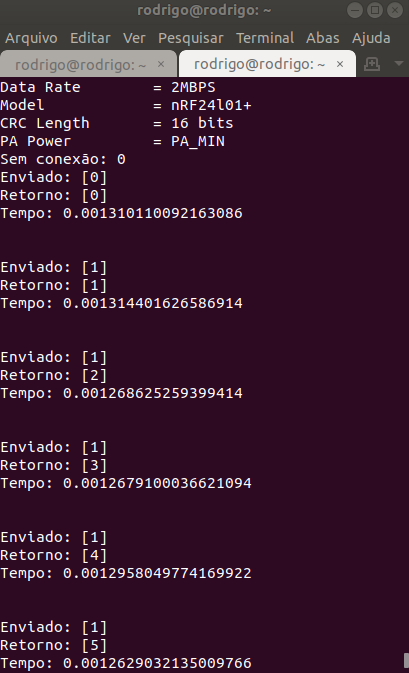
\includegraphics[width=\textwidth]{tx.png}
        \caption{Imagem do resultado do código de envio da \emph{flag} do Totem 1 para o Totem 2, mostrando o que foi enviado, do retorno de confirmação da recepção do Totem 2 e o tempo do processo.}
          \label{tx}
      \end{subfigure}
        \hfill
      \begin{subfigure}{0.49\textwidth}
        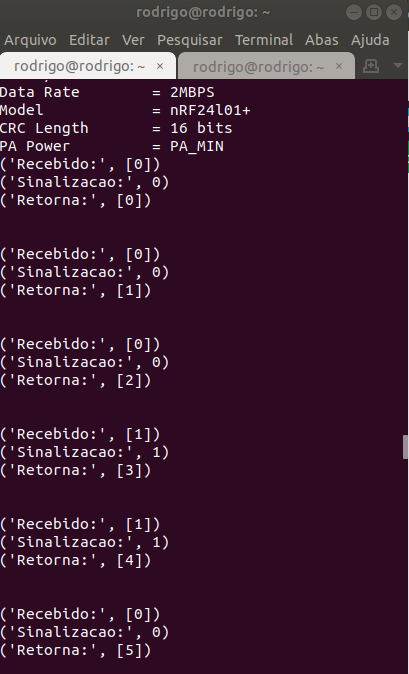
\includegraphics[width=\textwidth]{rx.png}
        \caption{Imagem do resultado do código de recebimento da \emph{flag} no Totem 2, mostrando a mensagem que foi recebida, envio de um retorno para confirmar que a mensagem foi recebida e o tempo do processo.}
          \label{rx}
      \end{subfigure}
        \hfill
        \label{}
\end{figure} 

Para a \ref{tx}, o resultado obtido é mostrado primeiramente a mensagem transmitida, o retorno enviado pelo totem de recepção, no caso um contador, e também é mostrado o tempo desde o envio da mensagem até o recebimento da confirmação de recepção. Para a \ref{rx}, é mostrado o resultado da mensagem recebida pelo transmissor, o estado da sinalização para que o holofote esteja ligado ou desligado, sendo este valor 1 ou 0, respectivamente, e o contador como retorno para avisar ao transmissor que a mensagem foi recebida.
 
  \subsection{Controle de Infração}
  
De acordo com o Artigo $5^{\circ}$ Parágrafo $1^{\circ}$ da Resolução do CONTRAN 396/11 \cite{CONTRAN}, a velocidade a ser considerada para que a penalidade seja efetivada será o resultado de uma subtração da velocidade medida pelo equipamento pelo erro máximo admitido previsto na legislação metrológica em vigor, também presente na Resolução \cite{CONTRAN}.
   
 Após encontrar o valor da velocidade considerada, é feita uma comparação para saber se o veículo realmente está acima da velocidade da via, e se estiver, é calculado a porcentagem acima da velocidade da via para saber qual tipo de infração o condutor está cometendo, que de acordo com o Artigo 218 do Código de Trânsito Brasileiro (CTB) \cite{CTB} temos 3 (três) tipos de infração, sendo elas a infração média, onde o veículo está no máximo acima 20\%, grave quando o veículo está entre 20 a 50\% e gravíssima quando o mesmo estiver acima dos 50\%.   
    
Para este processamento, após o cálculo da velocidade medida ela é convertida pelo valor tabelado para velocidade considerada, e faz as comparações com a velocidade máxima permitida da via, que normalmente é imposta pelo órgão de transito local.    

\subsection{Captura}
    
Caso o veículo detectado esteja acima da velocidade permitida, é realizado uma estimativa de tempo considerando a posição e a velocidade do veículo, que determinará quanto tempo o mesmo levará para chegar na região de captura da câmera, realizando o disparo da traseira do veículo.
    
Primeiramente foi determinado distância de captura de imagem que será entre 7 a 10 metros do radar para realização da captura da imagem. Após isso foi levantado os fatores determinantes para uma boa qualidade de imagem para detecção e reconhecimento da placa na distância determinada, sendo o tamanho da lente e também o diâmetro do sensor utilizado pelo aparelho, pois eles influenciam no ângulo de abertura da câmera, e como a distância de captura é considerável, quanto menor for o ângulo de abertura maior será a resolução da imagem captada. Outro fator importante é a utilização de uma lente varifocal, pois esta possibilita um ajuste automático do foco da lente de acordo com que os objetos se aproximam ou afastam dela. Com isso foi escolhido a câmera \emph{Hilook IPC-B620H-V/Z}, com captura de 2 MP e resolução de vídeo máxima de 1920 $\times$ 1280 a 30 fps. \par
Para realização dos testes a câmera foi configurada com uma qualidade de 1280 x 720 \emph{pixels} para uma qualidade boa e um tamanho de imagem menor em relação a qualidade máxima, uma quantidade alta de zoom para diminuir a quantidade de informação desnecessária da imagem e ter uma melhor visualização da placa do veículo, e por último também foi configurado em escala de cinza, diminuindo também o tamanho da imagem. A câmera foi instalada simulando sua posição na estrutura do radar, sendo a 3 metros de altura e a 7 metros de distância da região de captura. Para a conexão da câmera com a \emph{Raspberry Pi 3} foi utilizado um roteador com rede local, pelo fato da necessidade de ter uma alta taxa de transmissão devido ao envio de imagens para o servidor e da câmera necessitar de uma conexão estável com uma rede para estabelecer uma transmissão contínua. Utilizando a biblioteca \emph{OpenCV} e o protocolo de comunicação  \emph{Real Time Streaming Protocol} (RTSP) da pilha de protocolos \emph{Transmission Control Protocol/Internet Protocol} (TCP/IP), foi possível o acesso à câmera para realização da captura, como mostrado na Figura \ref{carro1} com o carro parado na região delimitada para o projeto.


\begin{figure}[H]
    \centering
    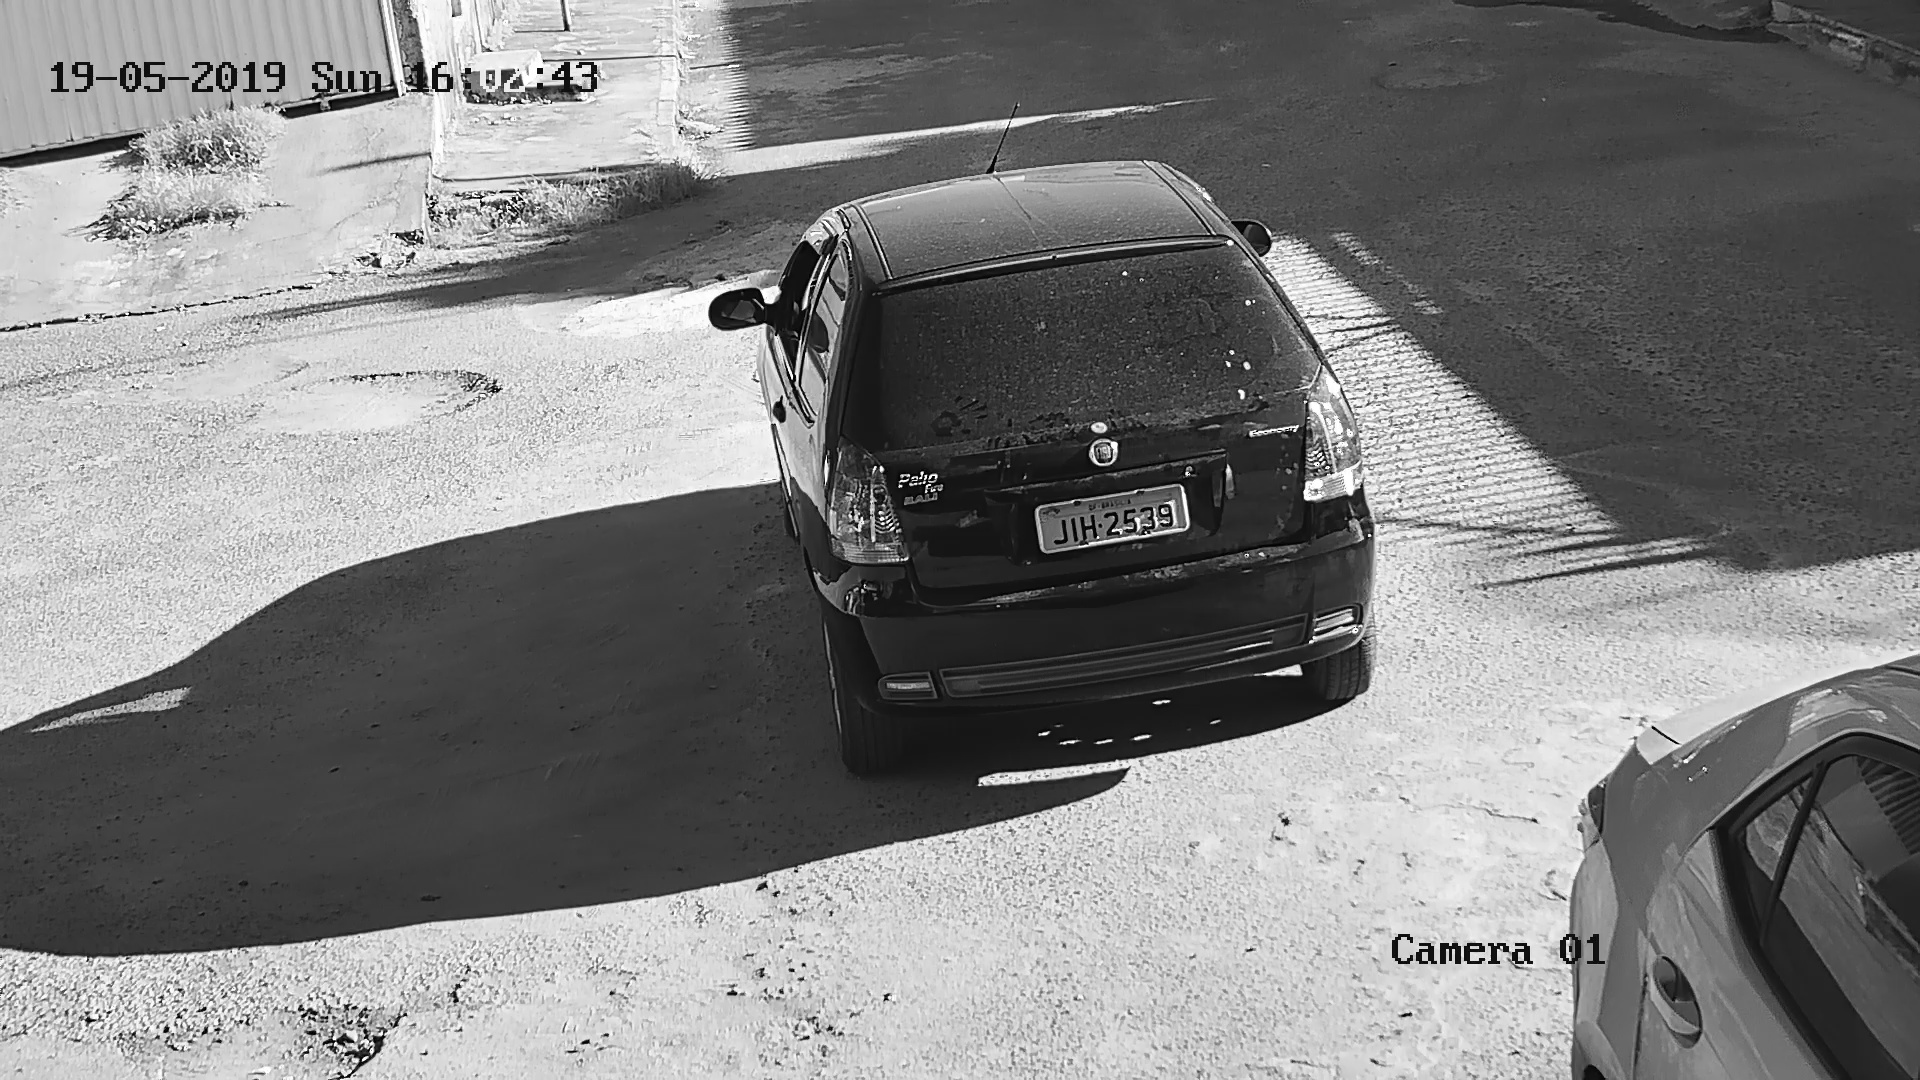
\includegraphics[scale=0.18]{carro1.jpg}
    \caption{Imagem capturada em escala de cinza pela câmera a 3 metros de altura e 7 metros de distância.}
    \label{carro1}
\end{figure}

Para saber o tempo de processamento de acesso à câmera e captura da imagem, foi utilizado a função \emph{time.time()}, que delimitando um início e um final no código é retornado o tempo limitado. O resultado para abertura da câmera é em torno de 1 s, e para captura da câmera este tempo variou em torno de 100 a 220 ms. Como a câmera será aberta apenas na inicialização, seu tempo de latência não será contabilizado no cálculo final, pelo fato do código após estar rodando não retornar na função. Como o tempo de latência máximo definido em \ref{tempo_latencia} é de 1.36 s, a captura em 200 ms satisfaz nosso requisito. Em relação ao tamanho da imagem gerada, houve uma variação em torno de 150 a 180 kB, sendo este valor muito menor que a imagem original da câmera em alta qualidade, aproximadamente de 1 MB.
A Tabela \ref{tabcap} relaciona o tamanho da imagem gerada com o tempo de captura.

\begin{table}[H]
\centering
\caption{Relação entre o tamanho da imagem pelo tempo de captura, onde se pode notar que quanto maior o tamanho da imagem, maior o tempo de captura.}
\label{undefined}
\begin{tabular}{|c|c|}
\hline
Tamanho da imagem (KB) & Tempo de captura (ms) \\ \hline
169                    & 120                   \\ \hline
173                    & 130                   \\ \hline
151                    & 110                   \\ \hline
179                    & 170                   \\ \hline
\label{tabcap}
\end{tabular}
\end{table}

    \subsection{Envio de dados para o servidor}
    
Para realizar o envio de dados para o servidor foi realizado previamente um estudo de caso para as rodovias brasileiras em geral, e notou-se que segundo o Departamento Nacional de Infraestrutura e Transporte (DNIT) \cite{DNIT} o fluxo médio das grandes rodovias é de aproximadamente 60 mil veículos por dia, de onde cerca de somente 0.5\% desses veículos geram infrações, resultando em uma média de 300 veículos infratores por dia.

O servidor receberá alguns dados do veículo que estiver transitando acima do limite estabelecido na via. Foi definido que os dados enviados serão: 

    \begin{itemize}
        \item ID do radar: Identificação do equipamento utilizado, mediante numeração estabelecida pela entidade de trânsito. Este dado será do tipo inteiro.
        \item Velocidade regulamentada: Velocidade limite para  local da via determinada pelas normas do CONTRAN \cite{CONTRAN}. Este dado será do tipo inteiro.
        \item Velocidade medida: Velocidade  do veículo calculada pelo equipamento. Este dado será do tipo inteiro.
        \item Velocidade considerada: Velocidade medida subtraída pelo erro máximo admitido previsto na legislação metrológica. Este dado será do tipo inteiro.
        \item Infração: Natureza da infração cometida. Estes dados serão do tipo inteiro enviados por enumeração, onde 0, 1 e 2 correspondem respectivamente a média, grave e gravíssima.
        \item Penalidade: Punição para o infrator, que neste caso sempre será a multa. Este dado será enviado do tipo \emph{boolean}, enviando sempre \emph{True}.
        \item Data e hora: A data e hora da infração será enviado no formato rfc3339, utilizando a função \emph{timestamp}, que representa um ponto específico na linha do tempo e leva em consideração o fuso horário em questão \emph{Universal Time Coordinated} (UTC). 
        \item Imagens: As imagens tanto em escala de cinza do carro quanto a imagem pré processada para reconhecimento da placa serão enviadas no formato base64, método para codificação de dados para transferência na Internet.
        \item Câmera: Retorna se a câmera está ou não funcionando corretamente. Este dado será dado por 1 bit inteiro sendo 1 para funcionando e 0 para caso ocorra falha.
        \item \emph{Raspberry}: Retorna se a \emph{Raspberry Pi 3} está ou não funcionando corretamente. Este dado será dado por 1 bit inteiro sendo 1 para funcionando e 0 para caso ocorra falha.
        \item USRP: Retorna se o USRP está ou não funcionando corretamente. Este dado será dado por 1 bit inteiro sendo 1 para funcionando e 0 para caso ocorra falha.
        \item Funcionamento do radar: Retorna se o radar em geral está funcionando corretamente. Este dado será dado 1 para funcionando e 0 para caso ocorra falha.
        \end{itemize} 
        
       
 O protocolo que fará comunicação entre a \emph{Raspberry Pi 3} e o servidor será o \emph{Hypertext Transfer Protocol} (HTTP), da pilha de protocolos TCP/IP. O pacote de dados será feito em \emph{JavaScript Object Notation} (JSON), pois é uma formatação leve de troca de dados com serviço web. Para o teste de envio para o servidor, foram gerados valores aleatórios dentro do formato de cada um dos objetos que será enviado, e foi feito um \emph{loop} para que o código rodasse cinco vezes mostrando o código de estado de conexão HTTP, o tempo de envio do pacote para o servidor e o tamanho do pacote que será enviado em \emph{Bytes}. Para a conexão ser realizada, foi utilizada a biblioteca \emph{requests} com a função \emph{post}, direcionando a url do servidor que receberá os dados. Os resultados da conexão se encontram na Figura \ref{servidor}
 
  \begin{figure}[H]
    \centering
    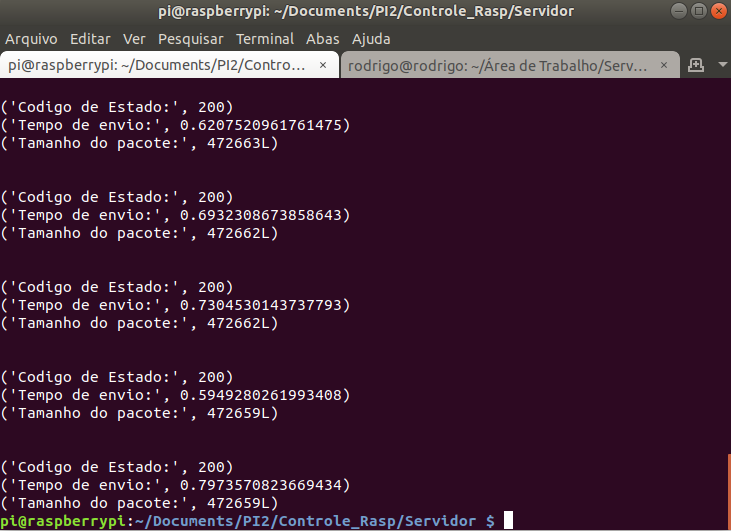
\includegraphics[scale=0.50]{servidor.png}
    \caption{Resultados do envio de pacote de dados para o servidor, mostrando o código de estado, o tempo de envio e o tamanho do pacote em \emph{Bytes}.}
    \label{servidor}
\end{figure}

O estado do código de conexão HTTP com o servidor retornou o valor de 200 , indicando que a requisição foi bem sucedida (OK) \textcolor{red}{13}, o tempo de envio é o resultando de todo o processamento de criação do pacote, envio para o servidor e retorno do estado HTTP e o tamanho do pacote resultante foi de 472 KB.

\section{Processamento de imagem}

Este processo tem como objetivo tratar a imagem capturada pela câmera de modo que possa ser reconhecido a placa do veículo, facilitando no reconhecimento dos caracteres que será feito pelo servidor. Ao final deste processo serão geradas duas imagens, uma contendo apenas a transformação de escala em cinza e a outra imagem será da placa a ser processada.
%%diagrama do processo
\begin{figure}[H]
    \centering
    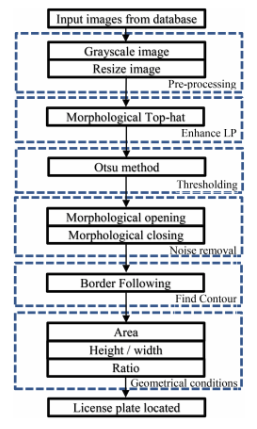
\includegraphics[scale = 0.6]{procimagpng.png}    \caption{Procedimentos e operações morfológicas para localização de placas de carro em imagens. Fonte \cite{Localisation}.}
    \label{fig:proc_img}
\end{figure}
A Figura \ref{fig:proc_img} trata da sequência de operações relacionadas a localização da placa de carro em uma imagem. 

%\begin{figure}[H]
  %  \centering
  %  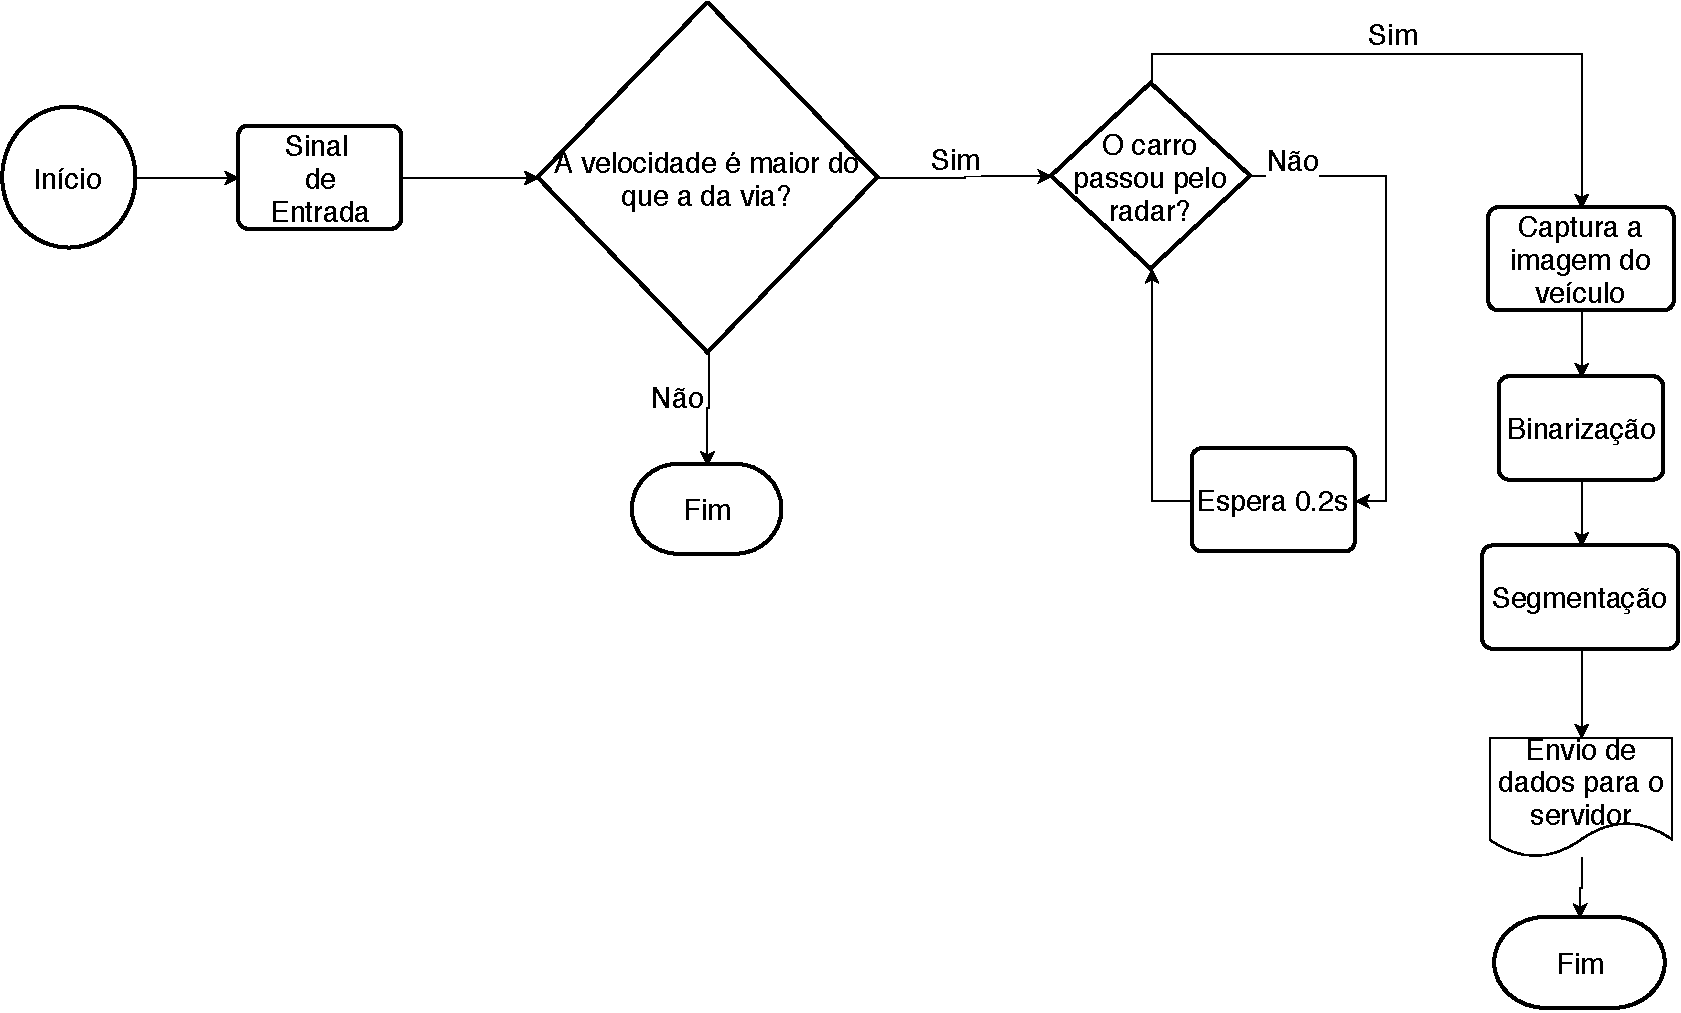
\includegraphics[scale=0.4]{Diagrama_logico_imagem.pdf}
  %  \caption{Etapas do processamento de imagem a serem realizadas e seus elementos responsáveis pela execução. A câmera faz a aquisição da imagem, a \emph{Raspberry Pi 3} faz o pré-processamento, segmentação e representação, e o servidor realiza o reconhecimento da placa. \textcolor{red}{10}} 
  %  \label{processamento_imagem}
%\end{figure}

\begin{itemize}
    \item \emph{Grayscale image}: Consiste em transformar a imagem em escala de cinza. 
    \item \emph{Top Hat}: Extração de elementos e detalhes da imagem, consistindo na subtração da imagem obtida na primeira etapa após uma operação de abertura com elemento estruturante no formato de um retângulo.
    \item Otsu \emph{method}: Processo de binarização através da técnica de Otsu que visa calcular o histograma de uma imagem e tomar como limiar. Para um processo de binarização, a metade do índice de dois picos para então usar este valor como limite. 
    \item \emph{Morphological opening/closing}: Remoção de ruído, através da sequência de abertura e fechamento para que objetos que não tem correspondência com o formato da placa sejam filtrados. 
    \item \emph{Border following}: Imagem foi varrida em busca de objetos que tem estrutura semelhante ao padrão utilizado nas outras etapas, destacando-os em seguida através de um algoritmo detector de borda, mais precisamente, o algoritmo \emph{Canny edge}. 
\end{itemize}
    
Todas as estapas foram implementadas através da plataforma OpenCV na linguagem de programação Python \cite{Localisation} \cite{Gonzalez}.


\subsubsection{Transformação para escala de cinza}
A escala de cinza é a transformação de uma imagem colorida, em que cada pixel é transformado em um valor que corresponde a uma escala do branco ao preto, diminuindo a quantidade de informação na imagem que não é útil para as sequências das operações. Esta transformação foi feita diretamente pelas configurações da câmera, não sendo necessário nenhum comando no código para o processamento do mesmo. Uma imagem com três canais de cores forma, RGB, por exemplo, endereça cada pixel através de duas dimensões sendo que cada elemento contém três valores, formando, assim, uma matriz com tamanho $M\,x\,N\,x\,P$ sendo P um vetor de três posições. Para um imagem com resolução de 1920 por 1080 pixels têm-se uma matriz com $1920\,x\,1080\,x\,3$ o que implica, em um objeto, de tamanho 6220800 enquanto que uma imagem em escala de cinza condiz com um objeto com tamanho 2073600. Outro ponto condicionado a utilização de imagens em escala de cinza é o efeito de operações morfológicas de acordo com \cite{Localisation}. As Figuras \ref{cinza} e \ref{original} mostram a transformação para escala de cinza de uma imagem colorida capturada pela câmera. 

\begin{figure}[H]
    \centering
     \begin{subfigure}{0.8\textwidth}
        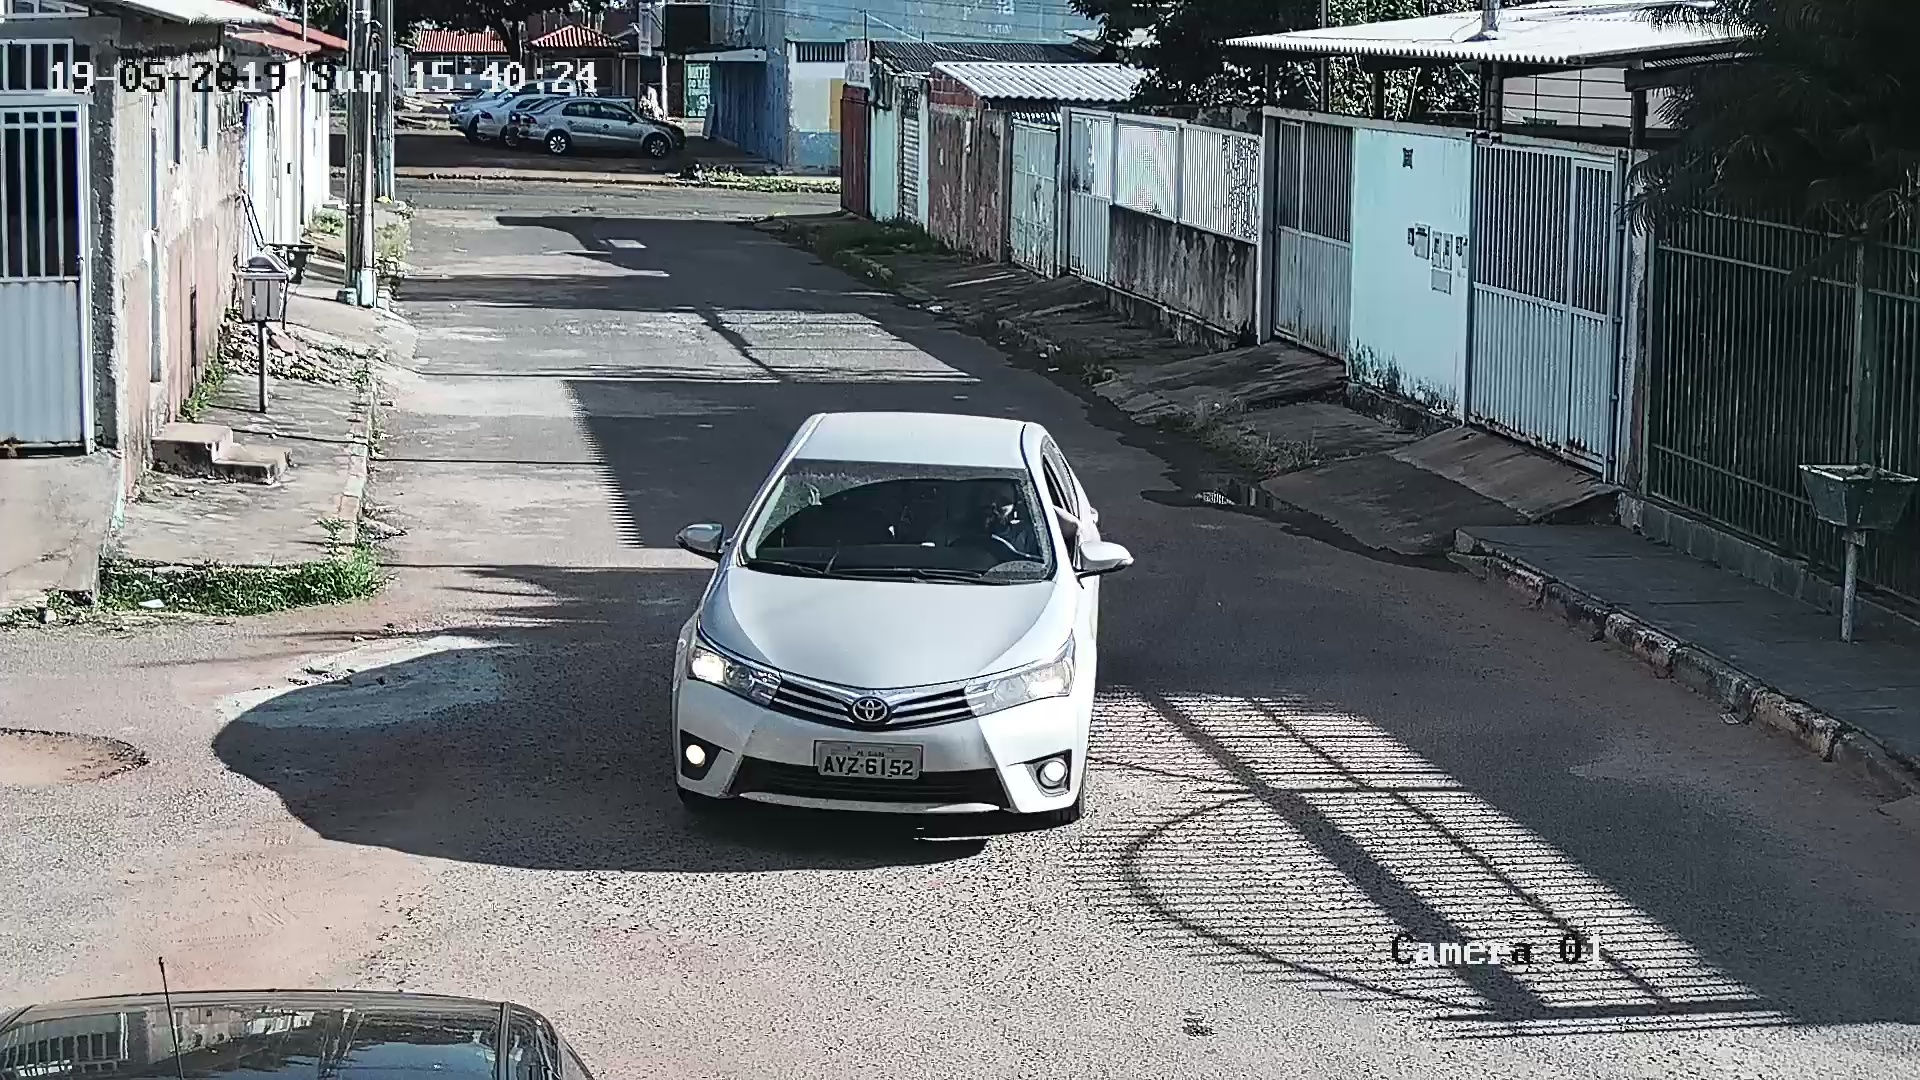
\includegraphics[width=\textwidth]{transforma2.jpg}
        \caption{Imagem original}
          \label{original}
      \end{subfigure}
        \hfill
      \begin{subfigure}{0.8\textwidth}
        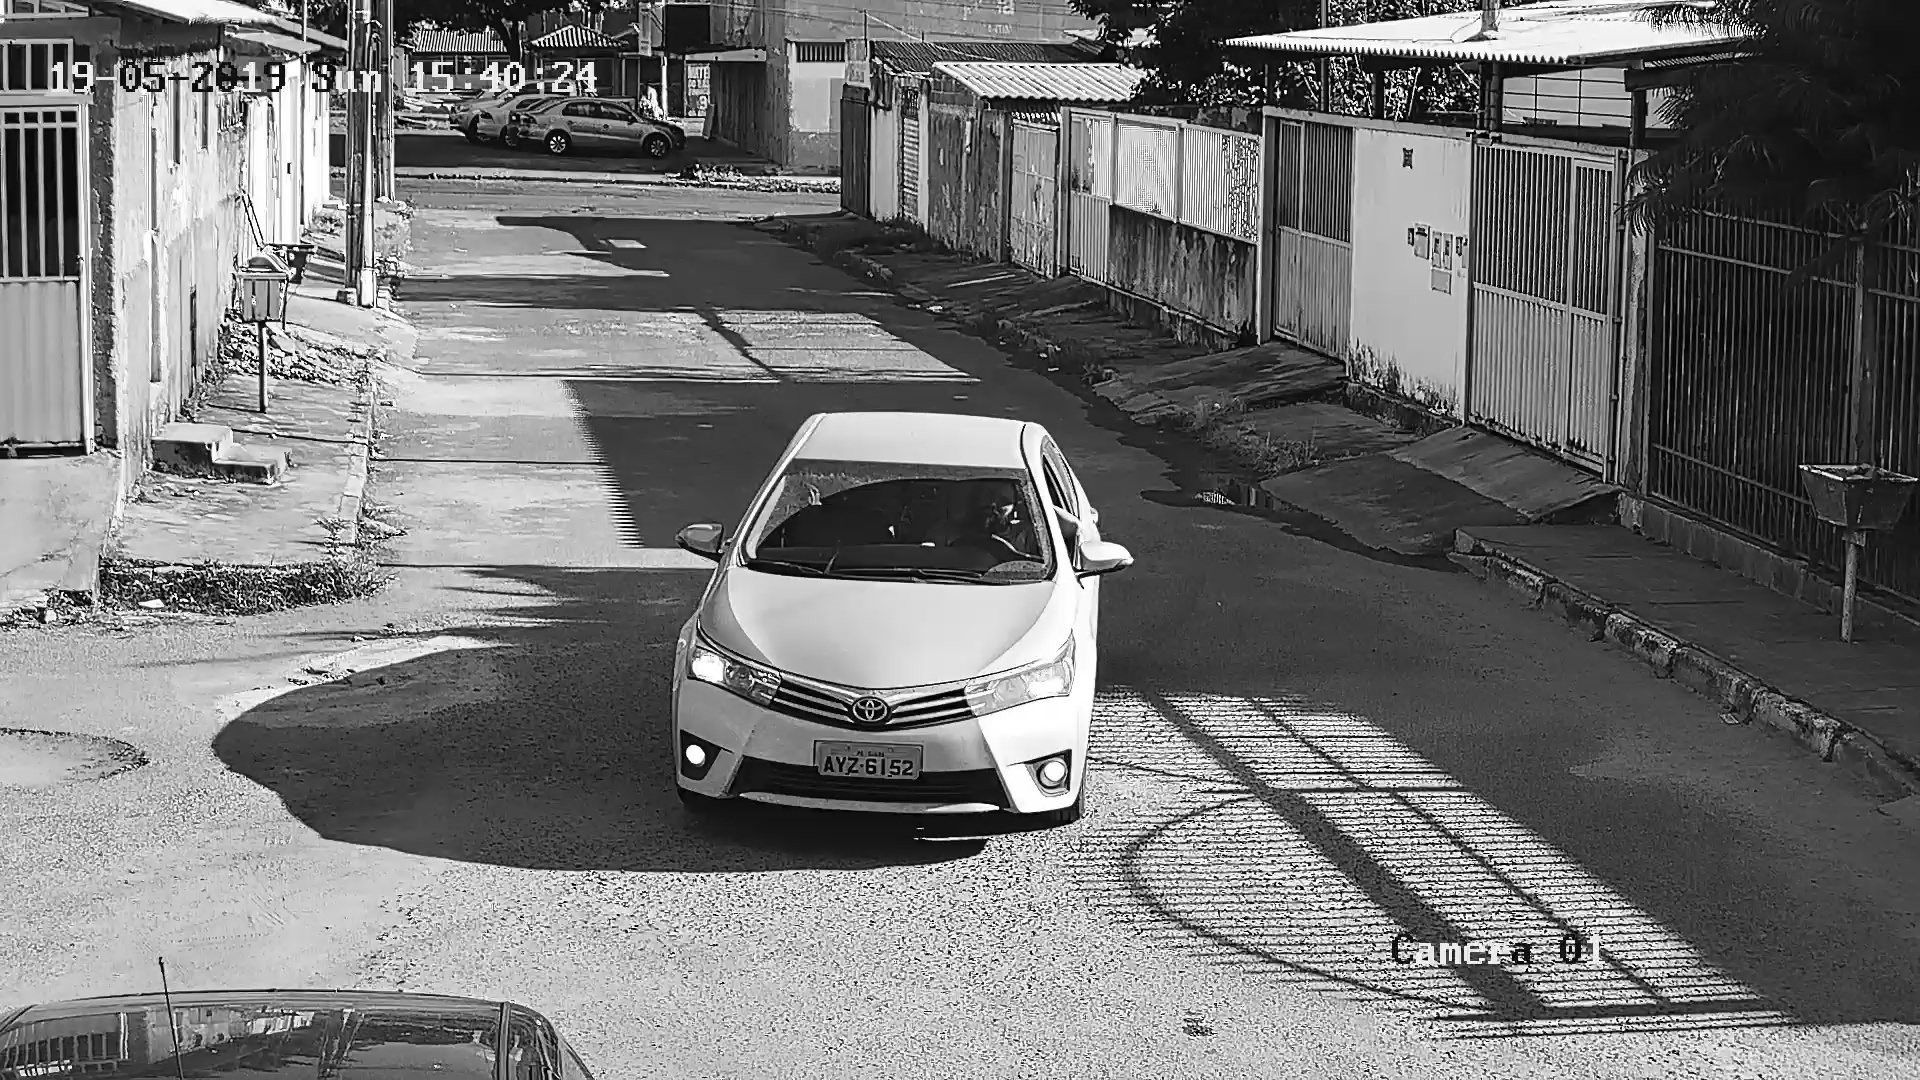
\includegraphics[width=\textwidth]{transforma2_1.jpg}
        \caption{Imagem original transformada em escala de cinza}
          \label{cinza}
      \end{subfigure}
        \hfill
       
\end{figure} 


\subsubsection{Binarização}
A partir de um aplicação de um limiar na imagem com escala em cinza, os \emph{pixels} com valores maiores que este limiar recebem o valor máximo da escala de cinza e os \emph{pixels} com valor menor que o limiar, recebem o valor mínimo  \cite{Gonzalez}.

\subsection{Resultados após processamento de imagem}


Na figura \ref{fig1:demarcada} foram demarcados vários elementos para tentar reduzir a quantidade de objetos, aplicando um filtro de borramento na imagem original para diminuir a quantidade de transições entre objetos candidatos a placa de carro e o fundo da imagem. A próxima etapa a ser feita é classificar o objeto na imagem em placa e não placa de carro, para, em seguida realizar o reconhecimento de caracteres.
Como elemento estruturante para as operações morfológicas foi utilizado um retângulo calculado de acordo com as especificações da câmera, sendo imagem com resolução de 1290 por 720 \emph{pixels} a uma distância aproximada de 10 m . Com ângulo de abertura horizontal e vertical de 34º e 19º, respectivamente, ocasiona em um plano com dimensionamentos de acordo com as Eqs. \ref{dimensoes1}:
\begin{equation}
    2\,d\,cos(\theta_{h} /2) = 19,12 m, 
    2\,d\,cos(\theta_{v} /2) = 19,72 m.
    \label{dimensoes1}
\end{equation}
As Eq. \ref{dimensoes1} permitem mensurar a densidade linear de pixels por metro, sendo, 66,93 pixels/m para a horizontal e 36,5 pixels/m para a vertical.
Sabendo-se que a dimensão da placa do carro é de 0,4 m por 0,15 m estimou-se o tamanho do elemento estruturante multiplicando-se a densidade de pixels obtida com o tamanho da placa obtendo-se uma matriz de tamanho 27 por 5, esse tamanho foi utilizado para formar um elemento estruturante de formato de um retângulo para ser utilizado na aplicação da operação morfológica \emph{Top Hat}. 

\begin{figure*}[t!]
     \centering
     
     \begin{subfigure}{0.7\textwidth}
         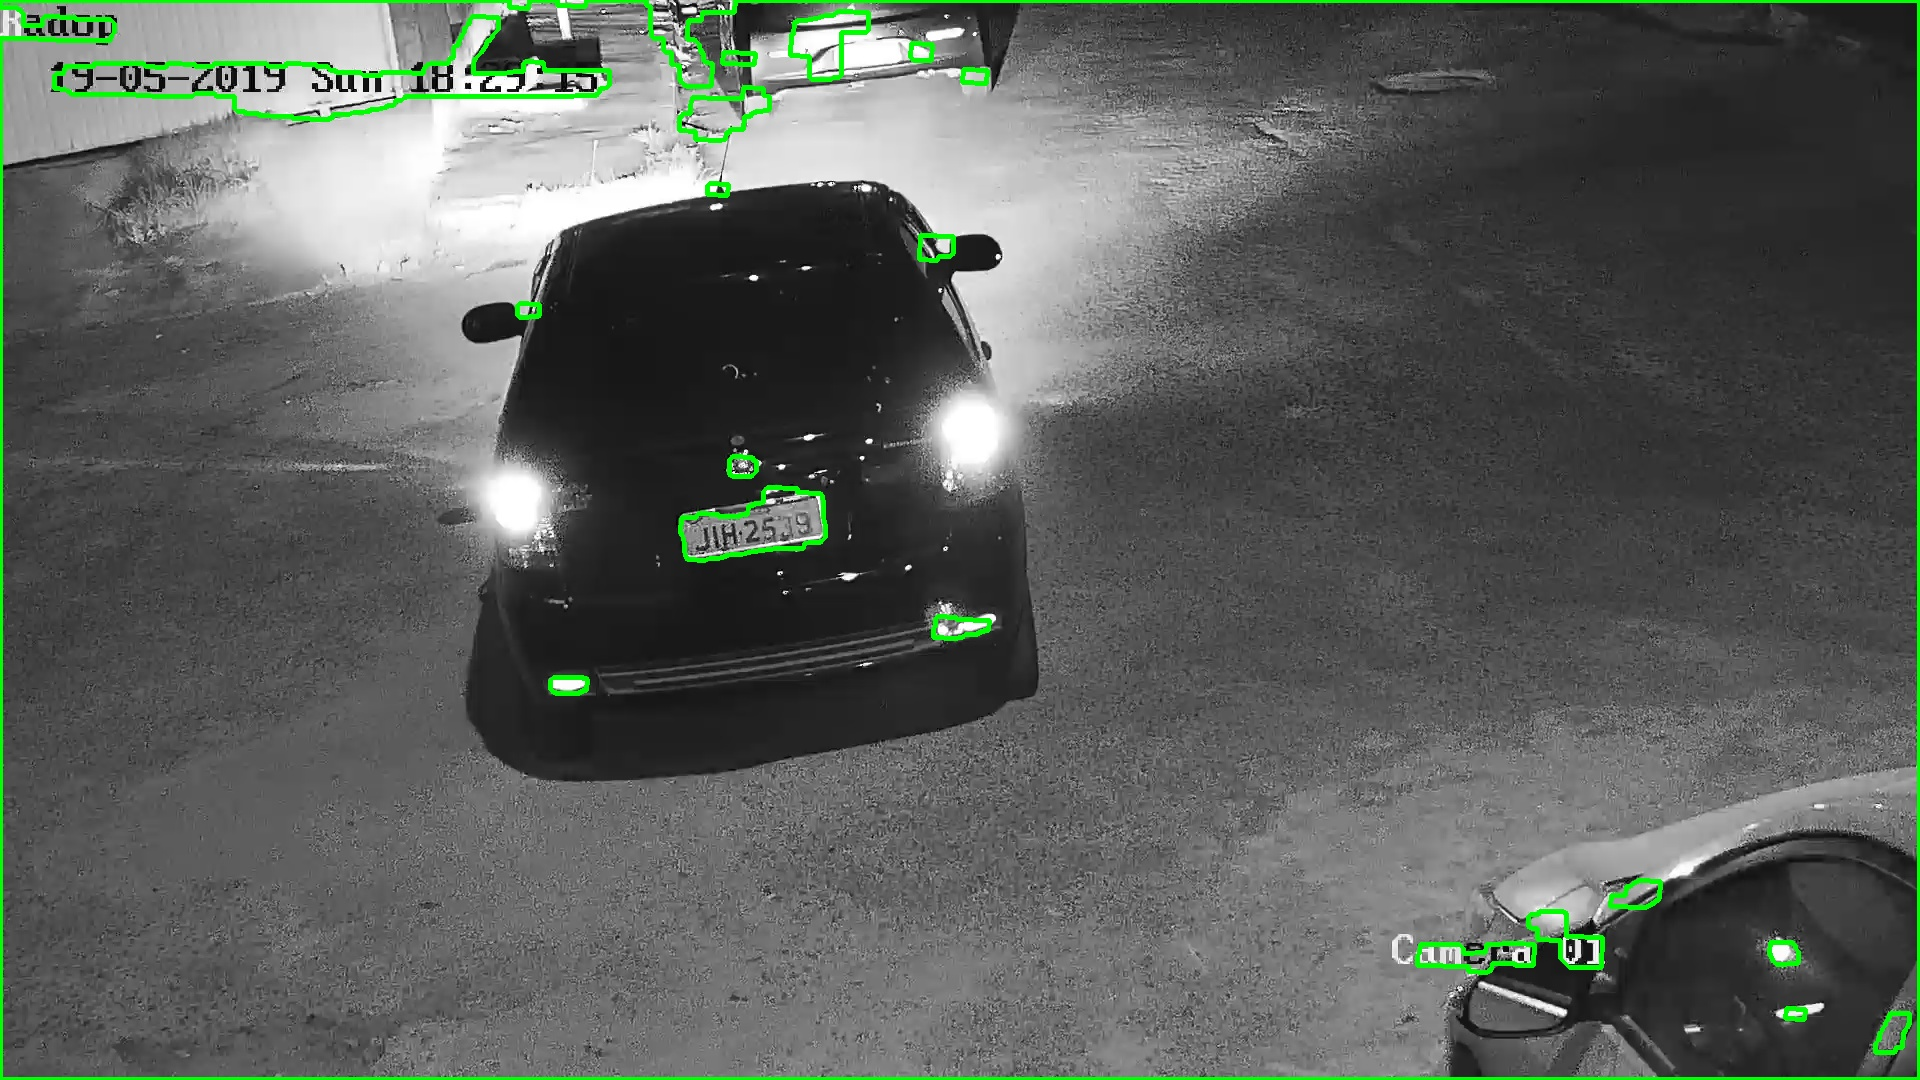
\includegraphics[width=\textwidth]{img_origin_n.jpg}
         \caption{}
         \label{fig1:demarcada}
     \end{subfigure}

     \begin{subfigure}{0.7\textwidth}
         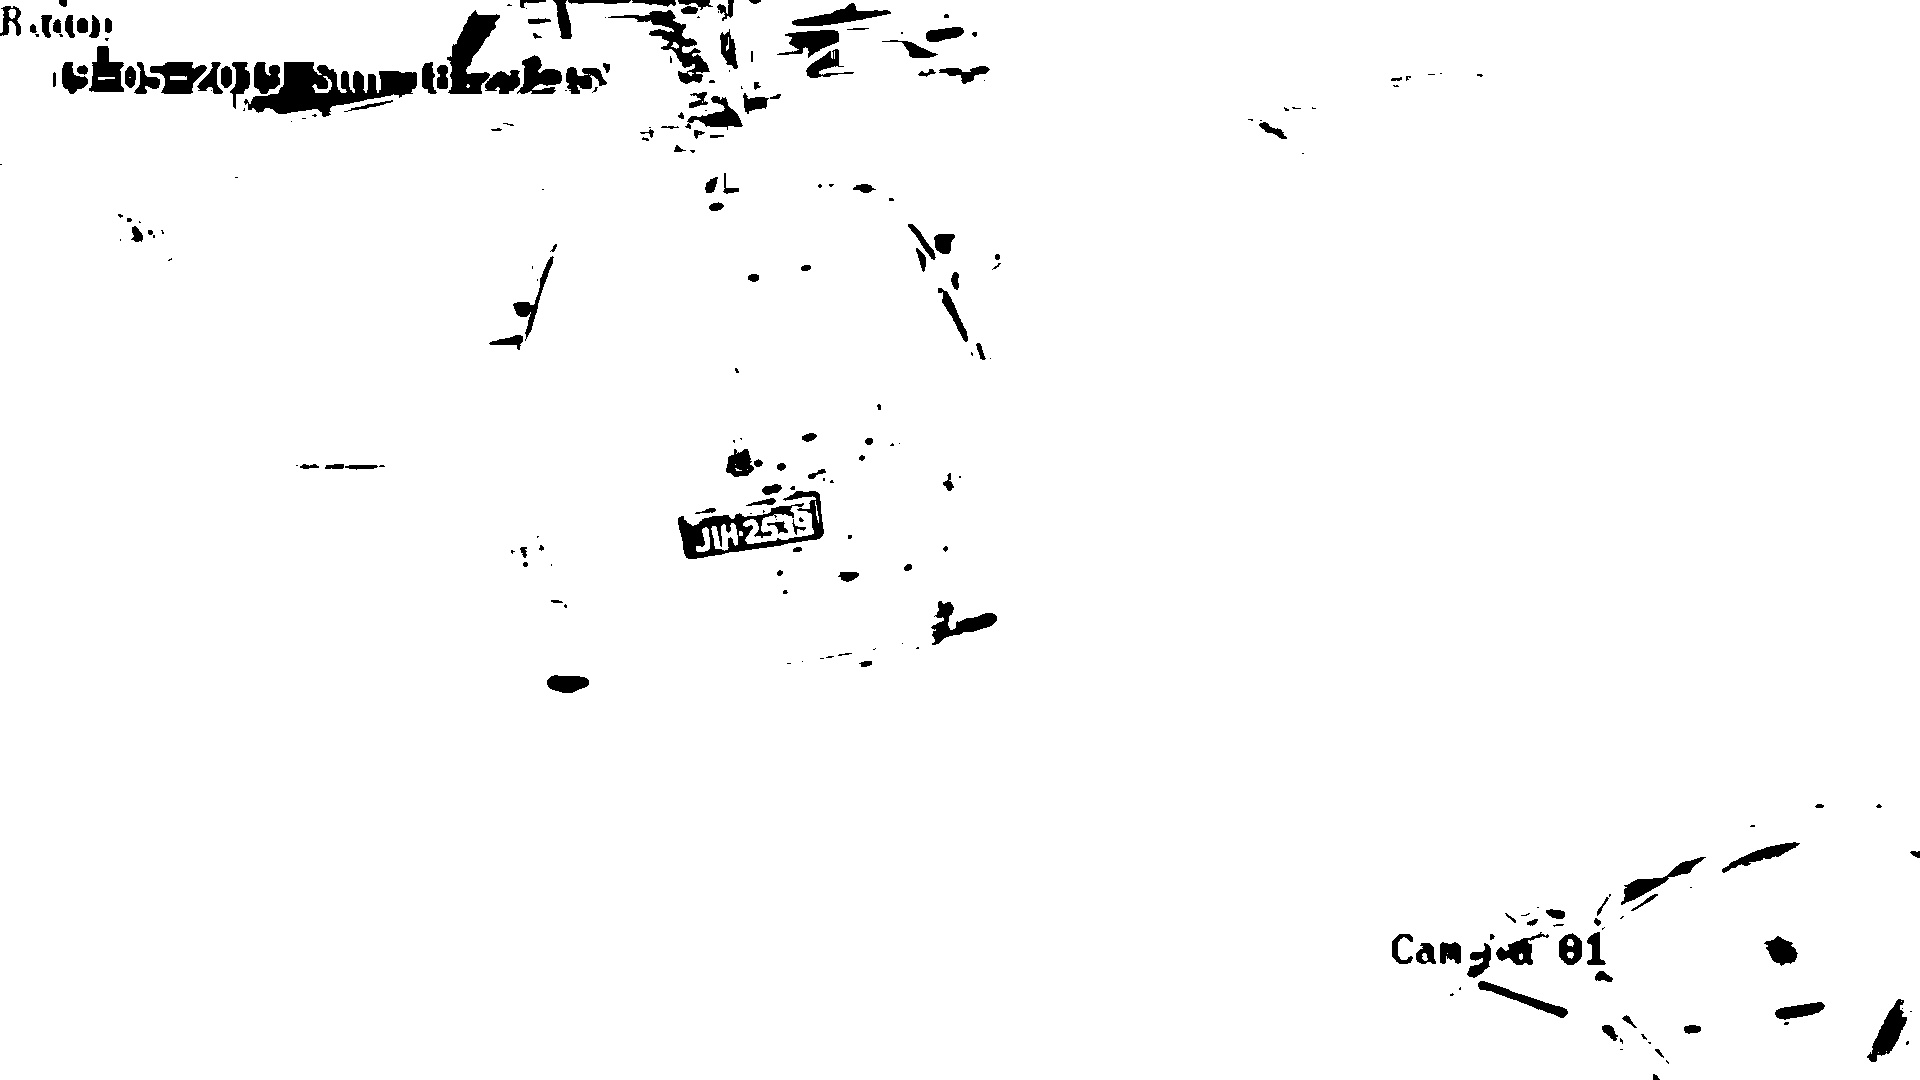
\includegraphics[width=\textwidth]{thr_n.jpg}
          \caption{}
         \label{fig2:thresh}
     \end{subfigure}

     \begin{subfigure}{0.7\textwidth}
         
\includegraphics[width=\textwidth]{op_cl_n.jpg}
          \caption{}
         \label{fig3:op_cl}
         
     \end{subfigure}
  \caption{\ref{fig1:demarcada} mostra marcação de locais possíveis onde pode haver uma placa de carro, \ref{fig2:thresh} corresponde a \emph{Top hat} mais binarização de Otsu e \ref{fig3:op_cl} mostra operações de abertura e fechamento.}
    \label{fig:three graphs}
\end{figure*}
